
\documentclass[11pt,a4paper]{article}
\usepackage[T1]{fontenc}
\usepackage{lmodern}
\usepackage{microtype}
\usepackage[margin=2.5cm]{geometry}
\usepackage{amsmath,amssymb}
\usepackage{booktabs,tabularx,longtable,array}
\usepackage{graphicx,float}
\usepackage[font=small,labelfont=bf,skip=6pt]{caption}
\usepackage{eurosym}
\usepackage{setspace}
\usepackage[dvipsnames]{xcolor}
\usepackage{tikz}
\usetikzlibrary{arrows.meta,positioning}
\usepackage[authoryear,round]{natbib}
\usepackage[colorlinks=true,linkcolor=MidnightBlue,citecolor=MidnightBlue,urlcolor=MidnightBlue]{hyperref}
\usepackage{fancyhdr}
\pagestyle{fancy}\fancyhf{}\renewcommand{\headrulewidth}{0pt}
\fancyfoot[C]{\footnotesize\thepage}
\setstretch{1.12}
\setlength{\parskip}{3pt}
\renewcommand{\floatpagefraction}{0.75}
\renewcommand{\topfraction}{0.85}

\title{\textbf{Gas Prices, Inflation Expectations and the German Yield Curve}\\[4pt]\large Evidence from the 2026 Iran War}
\author{Poctave}
\date{October 2026\\[2pt]\small Data to 9 October 2026}

\begin{document}
\maketitle
\thispagestyle{empty}

\begin{abstract}
\noindent I ask whether European natural gas prices move the German government bond curve, and whether they do so
through inflation expectations and the expected path of ECB policy. Using daily data from October 2014 to October
2026, I regress changes in inflation swaps, \euro{}STR overnight index swaps and Bund yields on returns of the Dutch
TTF gas contract, controlling for Brent and the euro, and I let the relationship differ across four regimes. It does
differ, sharply. Before 2021 gas barely moved Bund yields, and during the 2021--22 gas crisis higher gas prices came
with \emph{lower} yields. Since the Iran war began in March 2026, a 10\% rise in TTF has lifted the one-year
inflation swap by about 7bp, the expected policy rate one year ahead by 2 to 5bp and
the two-year Bund by about 4bp on the same day, while the 30-year yield has not moved: a bear flattening. A
break test with an unknown date puts the change in the first week of the war. Gas explains same-day curve moves, but
it does not forecast later ones out of sample. Its forecasting content is for realised inflation 6 to 12 months ahead.
\medskip

\noindent\textbf{Keywords:} natural gas, TTF, inflation swaps, ECB, Bund yield curve, regime dependence\\
\textbf{JEL:} E31, E43, E52, G12, Q43
\end{abstract}

\newpage
\section{Introduction}

On the first trading day after Iran closed the Strait of Hormuz, Dutch TTF gas jumped by about 40\% and the German
two-year yield rose 16bp over two days. The 30-year rose 6bp. That pattern, a large move at the short
end and a small one at the long end, repeated itself through the spring and summer of 2026 as the ECB raised its
deposit rate in June and again in September. Between 27 February and 9 October the two-year Bund went from
2.03\% to 3.09\% and the 30-year from 3.36\% to 3.85\%.

The story most market participants told was simple: gas drives inflation, inflation expectations drive rate-hike
expectations, and hike expectations drive the front end of the curve. This paper tests that chain link by link. I
care about two separate claims. The first is transmission: do gas moves show up, on the day, in inflation swaps,
\euro{}STR OIS and Bunds, after accounting for oil and the exchange rate? The second is predictability: does today's
gas move tell us anything about curve moves in the days and weeks that follow?

The short answers are yes and no. Transmission is strong in the war regime and absent or reversed before it. In the
war, a 10\% gas move lifts the one-year inflation swap by 6.9bp ($p<0.001$), the two-year Bund by
4.1bp ($p=0.003$) and leaves the 30-year unchanged (0.2bp, $p=0.886$), so the 2s30s slope falls by
about 3.9bp. In 2021--22 the same regression gives $-$1.2bp for the two-year Bund. Predictability, on the other
hand, is not there for the curve: local projections show no drift after the first day or two, and a gas-based
forecast of next week's Bund move does no better than assuming no change. Where gas does help is in forecasting
realised inflation, which responds with a lag of 6 to 12 months.

I think the regime result is the most useful one. It says the sign of the gas--rates relationship is set by how the
market expects the central bank to react, not by gas itself. When the ECB was seen as patient and gas as a threat to
growth, gas pushed yields down. Once the ECB had shown it would hike into an energy shock, the same gas move pushed
the front end up.

The rest of the paper is organised as follows. Section~\ref{sec:mech} lays out the mechanism. Section~\ref{sec:data}
describes the data and the cleaning it needed, including a timing problem in the Bundesbank series that would
otherwise produce spurious predictability. Section~\ref{sec:method} sets out the regressions. Section~\ref{sec:results}
reports the results, Section~\ref{sec:robust} the diagnostics, and Section~\ref{sec:disc} discusses what they mean
and where they stop. The appendix reports every OLS regression in full.

\section{Mechanism}\label{sec:mech}

Figure~\ref{fig:chain} shows the chain. Gas sets the marginal price of electricity in much of Europe and feeds into
household gas bills, fertiliser and industrial costs. Retail tariffs are regulated or contracted and reset slowly,
so the effect on consumer prices arrives months after the wholesale move. Markets do not wait for those prints.
Inflation swaps price expected HICP inflation directly: the one-year swap covers the next twelve months, and the 1y1y
forward covers the year after that, which is closer to the horizon the ECB targets. If the ECB is expected to respond
to higher expected inflation, \euro{}STR OIS rates rise, and with them the two-year Bund, which mostly tracks the
expected policy path. Long yields depend more on long-run growth, long-run inflation and term premia, so a policy shock
moves the short end more than the long end.

\begin{figure}[htbp]\centering
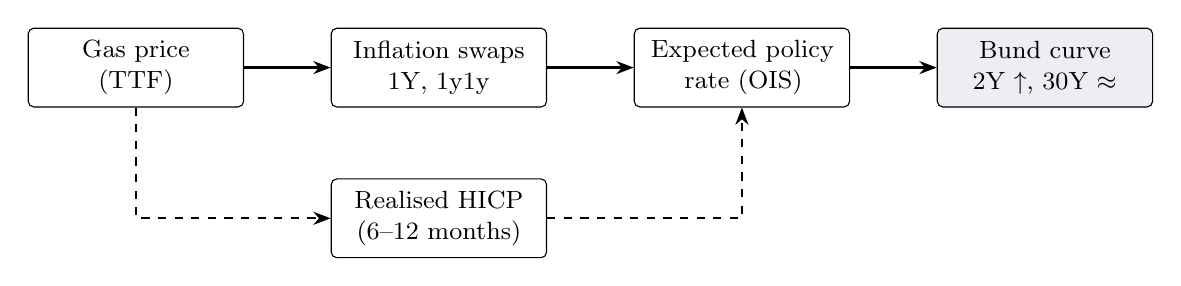
\begin{tikzpicture}[node distance=8mm and 11mm, every node/.style={font=\small},
  box/.style={draw, rounded corners=2pt, align=center, minimum height=10mm, text width=25mm, fill=white},
  arr/.style={-{Stealth[length=2.2mm]}, thick}]
\node[box] (gas) {Gas price\\(TTF)};
\node[box, right=of gas] (ils) {Inflation swaps\\1Y, 1y1y};
\node[box, right=of ils] (ois) {Expected policy\\rate (OIS)};
\node[box, right=of ois, fill=MidnightBlue!8] (bund) {Bund curve\\2Y $\uparrow$, 30Y $\approx$};
\node[box, below=9mm of ils] (hicp) {Realised HICP\\(6--12 months)};
\draw[arr] (gas) -- (ils);
\draw[arr] (ils) -- (ois);
\draw[arr] (ois) -- (bund);
\draw[arr, dashed] (gas) |- (hicp);
\draw[arr, dashed] (hicp) -| (ois);
\end{tikzpicture}
\caption{The transmission chain tested in this paper. Solid arrows: market prices that react on the day. Dashed: the
slower path through realised inflation, which the ECB reacts to at later meetings.}\label{fig:chain}
\end{figure}

Two forces work against this chain. A gas supply shock is also a growth shock, and weaker growth pushes yields down,
as does demand for safe assets in a crisis. Which force dominates depends on how the central bank is expected to
respond. The second problem is oil. The Hormuz closure hit oil and gas at once, and euro inflation swaps have
historically followed Brent more closely than gas, so any estimate of the gas effect has to control for oil.
\citet{adolfsen2026} add a further caution: in their BVAR, LNG supply shocks, which is what this war mostly is, move
euro-area inflation expectations less than pipeline supply shocks do.

\section{Data}\label{sec:data}

Table~\ref{tab:data} lists the series. The sample runs from October 2014 to 9 October 2026 at daily frequency.
\euro{}STR OIS starts in October 2019 and the one-year inflation swap in April 2022, so regressions involving them use
shorter samples. Bund yields come from the Bundesbank and are yields on the current (on-the-run) bond in each maturity
bucket. Everything else comes from LSEG.

\begin{table}[htbp]\centering\footnotesize
\caption{Data}\label{tab:data}
\begin{tabularx}{\textwidth}{@{}l l X l@{}}
\toprule
Series & Source / code & Definition & Start\\\midrule
TTF gas & LSEG TFMBMc1 & ICE Endex Dutch TTF front-month futures, EUR/MWh & 2014\\
Brent & LSEG LCOc1 & ICE Brent front-month futures, USD/bbl & 2014\\
EUR/USD, EUR/GBP & LSEG EUR=, EURGBP= & Spot mid & 2014\\
Inflation swap 1Y & LSEG EUCPIZ1Y=TWEB & Zero-coupon swap on euro-area HICP ex tobacco, 1 year & 2022\\
Inflation swap 1y1y & LSEG EUIL1YF1Y=R & One-year rate starting in one year & 2016\\
\euro{}STR OIS & LSEG EUREST1M/3M/1Y/2Y= & Overnight index swaps; 1y1y forward derived from 1Y and 2Y & 2019\\
Bund yields & Bundesbank BBSSY & Yields of current federal securities, 2Y to 30Y & 1993--2026\\
5Y swap spread & LSEG DE5IRS5Y=RR & 5Y swap rate minus 5Y Bund, bp & 2014\\
HICP & Eurostat & Euro-area index, 2025 = 100, not seasonally adjusted & 1999\\
\bottomrule
\end{tabularx}
\end{table}

Four data problems mattered. The file delivered as the ``1Y inflation swap'' is in fact the 1y1y forward; I relabelled
it and added the true one-year swap. The HICP file splices two index bases, which creates a fake 34\% drop in December
1999; I keep only the data on the current base. Front-month futures series jump when the contract rolls, so I identify
roll days from jumps in open interest (about twelve a year) and drop those returns.

The fourth problem is timing, and it is the one that would have done the most damage. The Bundesbank observes its
yields roughly half a trading day before the LSEG closes used for gas, swaps and OIS. Regressing the daily change in the
two-year Bund on the same-day and previous-day change in the two-year OIS gives coefficients of 0.49 and
0.53, and the correlation between the two series rises from 0.44 at one day to 0.67 at two days and 0.87
at five. Ignored, this mismatch makes yesterday's swap and gas moves look like they predict today's Bund move. I deal
with it by adding the previous day's market moves to every daily regression with a Bundesbank series on the left-hand
side, and by repeating the analysis at weekly frequency.

I split the sample into four regimes: 2014--21 (before the gas crisis, with the ECB at or below zero), July 2021 to
December 2022 (the gas crisis), January 2023 to 27 February 2026, and the Iran war from 2 March 2026. Table~\ref{tab:desc}
describes the daily changes. All series have fat tails (the excess kurtosis of the two-year Bund change is 15 in the
full sample) and volatility clusters, which is why every standard error in this paper is heteroskedasticity- and
autocorrelation-robust.

\begin{table}[htbp]\centering\footnotesize
\caption{Daily changes: full sample and Iran-war regime}\label{tab:desc}
\setlength{\tabcolsep}{5pt}
\begin{tabular}{@{}lccccccc@{}}
\toprule
Daily change & $N$ & s.d. & Excess kurt. & AC(1) & $N$ (war) & Mean (war) & s.d. (war)\\\midrule
TTF return (\\%) & 2906 & $4.35$ & $10.8$ & $0.02$ & 150 & $0.66$ & $5.39$\\
Brent return (\\%) & 2914 & $2.55$ & $13.9$ & $0.01$ & 150 & $0.34$ & $3.94$\\
ILS 1y1y (bp) & 2733 & $3.73$ & $9.2$ & $0.07$ & 157 & $0.30$ & $4.50$\\
OIS 1y1y (bp) & 1784 & $6.08$ & $4.4$ & $0.02$ & 157 & $0.82$ & $7.65$\\
Bund 2Y (bp) & 3041 & $4.12$ & $15.3$ & $-0.03$ & 157 & $0.68$ & $5.35$\\
Bund 10Y (bp) & 3041 & $4.52$ & $4.5$ & $-0.01$ & 157 & $0.50$ & $4.32$\\
Bund 30Y (bp) & 3041 & $4.61$ & $3.4$ & $-0.00$ & 157 & $0.31$ & $3.41$\\
2s10s (bp) & 3041 & $3.01$ & $4.4$ & $-0.03$ & 157 & $-0.18$ & $2.82$\\
\bottomrule
\end{tabular}
\par\vspace{4pt}\begin{minipage}{0.92\textwidth}\scriptsize\textit{Notes:} Full sample October 2014 to 9 October 2026 (shorter for OIS and swaps). The war regime starts on 2 March 2026. TTF and Brent returns exclude contract-roll days.\end{minipage}
\end{table}

\section{Empirical strategy}\label{sec:method}

\subsection{Transmission regressions}

Unit-root tests (Appendix Table~\ref{tab:ur}) show that all the series are non-stationary in levels and stationary in
first differences, and there is no robust cointegration between gas and yields (Table~\ref{tab:coint}). I therefore
work with changes. Let $\Delta y_t$ be the daily change in basis points of an inflation swap, OIS rate, Bund yield or
slope, and let $g_t$, $o_t$ and $e_t$ be 100 times the log change in TTF, Brent and EUR/USD. For series observed at the
LSEG close the regression is
\begin{equation}\label{eq:lseg}
\Delta y_t = \alpha + \beta\, g_t + \gamma\, o_t + \delta\, e_t + \varepsilon_t ,
\end{equation}
and for Bundesbank yields and slopes, which are observed earlier in the day,
\begin{equation}\label{eq:bbk}
\Delta y_t = \alpha + \sum_{j=0}^{1}\left(\beta_j\, g_{t-j} + \gamma_j\, o_{t-j} + \delta_j\, e_{t-j}\right) + \varepsilon_t ,
\end{equation}
in the spirit of \citet{dimson1979}. The total gas effect is $\beta$ in (\ref{eq:lseg}) and $\beta_0+\beta_1$ in
(\ref{eq:bbk}). Because $g_t$ is a log return in percent, the effect of a 10\% rise in TTF is $\beta \times 100\ln 1.1
\approx 9.53\,\beta$ basis points; this is the number I report in the text. Brent and EUR/USD enter as controls, not as
objects of interest.

All regressions are estimated by OLS separately in each regime. Standard errors are Newey--West with a Bartlett kernel
and $L=\lfloor 4(T/100)^{2/9}\rfloor$ lags \citep{neweywest1987}, which gives 4 lags in the war regime
($T=135$ for the Bund regressions) and 8 in the full sample ($T=2642$). The weekly version
uses Friday-to-Friday changes with 3 lags in the war regime ($T=32$). Weekly gas and Brent returns
are sums of the roll-cleaned daily returns, and for Bund series the weekly market window ends on Thursday, so it closes
before the Bundesbank's Friday observation.

To test whether the war changed the relationship I pool the full sample and interact every regressor with regime
dummies,
\begin{equation}\label{eq:inter}
\Delta y_t = \alpha + \sum_{r} \alpha_r D^r_t + \mathbf{x}_t'\boldsymbol\theta + \sum_{r\in\{\text{crisis},\,\text{war}\}} D^r_t\, \mathbf{x}_t'\boldsymbol\theta_r + \varepsilon_t ,
\end{equation}
where $\mathbf{x}_t$ holds the regressors of (\ref{eq:lseg}) or (\ref{eq:bbk}), and I test that the gas elements of
$\boldsymbol\theta_r$ sum to zero. I also run a Chow test at 2 March 2026 and a \citet{andrews1993} sup-Wald test that
searches for the break date over the middle 70\% of a 2023--26 sample. Because I test 20 dependent variables, I report
Holm-adjusted $p$-values \citep{holm1979} as well as raw ones.

\subsection{Channel, dynamics and forecasting}

To ask how much of the gas effect runs through inflation expectations, I estimate a serial mediation model
\begin{equation}\label{eq:med}
M_{1t} = a_1 g_t + \ldots,\qquad M_{2t} = a_2 g_t + d_{21} M_{1t} + \ldots,\qquad \Delta y_t = c' g_t + b_1 M_{1t} + b_2 M_{2t} + \ldots
\end{equation}
with $M_1$ the inflation swap, $M_2$ the OIS 1y1y and the same controls throughout. The indirect effects are
$a_1 b_1$, $a_2 b_2$ and $a_1 d_{21} b_2$. Confidence intervals come from a moving-block bootstrap. The daily version
stops at OIS, because all three series share the LSEG close; the full chain to the Bund runs at weekly frequency.

For dynamics I use local projections \citep{jorda2005},
\begin{equation}\label{eq:lp}
y_{t+h} - y_{t-1} = \alpha_h + \beta_h\, g_t + \gamma_h\, o_t + \delta_h\, e_t + \sum_{k=1}^{2}\left(\phi_{hk}\, g_{t-k} + \psi_{hk}\, \Delta y_{t-k}\right) + u_{t+h}, \quad h = 0,\ldots,20,
\end{equation}
and a predictive variant whose left-hand side starts after the impact day. I complement these with a VAR and Granger
tests, and with expanding-window out-of-sample forecasts of next week's change evaluated with the
\citet{clarkwest2007} test. Finally, for the first link of the chain I regress year-on-year HICP inflation on 12-month
changes in TTF and Brent (in euros) lagged $L=0,\ldots,12$ months.

\section{Results}\label{sec:results}

\subsection{Gas reaches inflation with a lag}

Oil and gas reach consumer prices on different clocks (Figure~\ref{fig:hicp}, Table~\ref{tab:hicp}). A 10\% rise in
Brent adds 0.30pp to year-on-year HICP inflation in the same month ($p=0.011$). The same rise in TTF adds nothing on
impact ($-$0.01pp), but its effect builds steadily to 0.21pp after nine months ($p=0.020$) and 0.24pp after a year
($p=0.007$). In a distributed-lag model of monthly inflation the gas lags are jointly significant ($p<0.001$), while
the first six months on their own are not ($p=0.068$). This is what one would expect from regulated retail tariffs, and
it matters for the rest of the paper: when gas jumps, the inflation the ECB will see arrives at the horizon it targets.

\begin{table}[htbp]\centering\footnotesize
\caption{Energy prices and realised inflation: HICP y/y on lagged 12-month energy price changes}\label{tab:hicp}
\setlength{\tabcolsep}{5pt}
\begin{tabular}{@{}lcccccc@{}}
\toprule
Lag (months) & TTF, pp & $p$ & Brent, pp & $p$ & $R^2$ & $N$\\\midrule
0 & $-0.01$ & 0.918 & $0.30$ & 0.011 & $0.17$ & 130\\
3 & $0.10$ & 0.216 & $0.20$ & 0.076 & $0.33$ & 127\\
6 & $0.15$ & 0.065 & $0.17$ & 0.185 & $0.50$ & 124\\
9 & $0.21$ & 0.020 & $0.04$ & 0.767 & $0.58$ & 121\\
12 & $0.24$ & 0.007 & $-0.09$ & 0.471 & $0.56$ & 118\\
\bottomrule
\end{tabular}
\par\vspace{4pt}\begin{minipage}{0.92\textwidth}\scriptsize\textit{Notes:} Each row is a regression of euro-area HICP inflation (y/y, pp) on the 12-month log change in TTF and Brent (in euros), both lagged $L$ months; coefficients scaled to a $+10\%$ change. Monthly data from December 2015; Newey--West standard errors (12 lags).\end{minipage}
\end{table}

\begin{figure}[htbp]\centering
\includegraphics[width=0.82\textwidth]{figs/f5_hicp_lag_scan.pdf}
\caption{Effect of a 10\% rise in energy prices on euro-area HICP inflation (y/y), by months of lag. Brent's effect
is immediate and fades; TTF's builds over a year.}\label{fig:hicp}
\end{figure}

\subsection{Same-day transmission in the war}

Tables~\ref{tab:war} and~\ref{tab:warb} report the war-regime regressions in full. Three things stand out. First, gas moves the front end.
The two-year Bund rises 4.1bp per 10\% gas move, almost all of it on the same day ($\hat\beta_0=0.404$ per 1\%
against $\hat\beta_1=0.024$). The effect falls with maturity: 2.0bp at five years, 1.3bp at ten and
0.2bp at thirty. Second, the fit is far better than in normal times. The two-year Bund regression has an $R^2$ of
0.40 (adjusted 0.37, robust $F=20.9$), against 0.02 in the full sample. For the one-year
inflation swap the $R^2$ is 0.67, and for the OIS 1y1y 0.58.

Third, oil is doing a lot of the work in the swap markets. Brent's effect on the one-year inflation swap is
17.4bp per 10\%, against 6.9bp for gas, and on the OIS 1y1y it is 11.4bp against 2.3bp.
For the Bund, Brent's effect is split evenly between the same day ($\hat\gamma_0=0.303$) and the previous day
($\hat\gamma_1=0.301$, $p=0.039$). That fits the timing problem described above: Brent settles in the London
evening, after the Bundesbank has taken its snapshot, so part of each day's oil move reaches the Bund series a day later. Gas keeps a
significant effect on the two-year Bund after all of this. The raw $p$-value is $p=0.003$; after Holm correction
it is 0.036 within the 13 rate series and 0.057 across all 20 series tested, so it sits right at the
conventional threshold under the strictest correction. The weekly estimate, which is free of the timing issue, is
3.6bp ($p=0.001$; Appendix Table~\ref{tab:w_war}).

\begin{table}[htbp]\centering\footnotesize
\caption{OLS transmission regressions, Iran-war regime (daily, 2 March -- 9 October 2026), part 1: expectations and yields}\label{tab:war}
\setlength{\tabcolsep}{5pt}\renewcommand{\arraystretch}{1.05}
\begin{tabular}{@{}l*{4}{c}@{}}
\toprule
\multicolumn{5}{@{}l}{\textit{Panel A. Inflation and policy expectations}}\\
 & ILS 1Y & ILS 1y1y & OIS 1y1y & OIS 2Y\\\midrule
$g_t$ (TTF) & $0.722^{***}$ & $0.186^{**}$ & $0.244^{**}$ & $0.217^{**}$\\
 & $(0.196)$ & $(0.082)$ & $(0.122)$ & $(0.107)$\\
$o_t$ (Brent) & $1.825^{***}$ & $0.516^{***}$ & $1.201^{***}$ & $0.991^{***}$\\
 & $(0.171)$ & $(0.074)$ & $(0.145)$ & $(0.128)$\\
$e_t$ (EUR/USD) & $1.484$ & $-0.964$ & $-2.105$ & $-1.446$\\
 & $(1.543)$ & $(0.771)$ & $(1.613)$ & $(1.421)$\\
Constant & $0.898$ & $-0.061$ & $0.460$ & $0.420$\\
 & $(0.565)$ & $(0.230)$ & $(0.325)$ & $(0.284)$\\
\cmidrule(l){2-5}
TTF total, bp per $+10\%$ & $6.88^{***}$ & $1.77^{**}$ & $2.32^{**}$ & $2.07^{**}$\\
 & $(1.87)$ & $(0.78)$ & $(1.16)$ & $(1.02)$\\
$R^2$ & 0.672 & 0.425 & 0.578 & 0.579\\
Adjusted $R^2$ & 0.665 & 0.412 & 0.569 & 0.570\\
Robust $F$ (all slopes) & 186.3$^{***}$ & 44.5$^{***}$ & 92.7$^{***}$ & 80.0$^{***}$\\
Residual s.e. (bp) & 6.96 & 3.30 & 5.03 & 4.16\\
Durbin--Watson & 2.17 & 2.17 & 2.34 & 2.31\\
HAC lags & 4 & 4 & 4 & 4\\
Observations & 142 & 143 & 143 & 143\\
\addlinespace[4pt]
\multicolumn{5}{@{}l}{\textit{Panel B. Bund yields}}\\
 & Bund 2Y & Bund 5Y & Bund 10Y & Bund 30Y\\\midrule
$g_t$ (TTF) & $0.404^{***}$ & $0.248^{***}$ & $0.183^{*}$ & $0.040$\\
 & $(0.105)$ & $(0.089)$ & $(0.094)$ & $(0.087)$\\
$g_{t-1}$ & $0.024$ & $-0.037$ & $-0.044$ & $-0.020$\\
 & $(0.095)$ & $(0.083)$ & $(0.086)$ & $(0.071)$\\
$o_t$ (Brent) & $0.303^{*}$ & $0.333^{***}$ & $0.269^{**}$ & $0.201^{**}$\\
 & $(0.164)$ & $(0.125)$ & $(0.118)$ & $(0.088)$\\
$o_{t-1}$ & $0.301^{**}$ & $0.293^{***}$ & $0.285^{***}$ & $0.174^{**}$\\
 & $(0.146)$ & $(0.105)$ & $(0.092)$ & $(0.076)$\\
$e_t$ (EUR/USD) & $1.200$ & $1.107$ & $1.356$ & $1.135$\\
 & $(0.834)$ & $(0.810)$ & $(0.839)$ & $(0.777)$\\
$e_{t-1}$ & $-1.862^{*}$ & $-1.834^{**}$ & $-1.206$ & $-0.461$\\
 & $(1.053)$ & $(0.830)$ & $(0.776)$ & $(0.848)$\\
Constant & $0.530^{*}$ & $0.467^{*}$ & $0.434$ & $0.274$\\
 & $(0.313)$ & $(0.276)$ & $(0.270)$ & $(0.263)$\\
\cmidrule(l){2-5}
TTF total, bp per $+10\%$ & $4.08^{***}$ & $2.01$ & $1.32$ & $0.19$\\
 & $(1.37)$ & $(1.22)$ & $(1.39)$ & $(1.30)$\\
$R^2$ & 0.397 & 0.377 & 0.302 & 0.146\\
Adjusted $R^2$ & 0.369 & 0.348 & 0.269 & 0.106\\
Robust $F$ (all slopes) & 20.9$^{***}$ & 21.5$^{***}$ & 13.6$^{***}$ & 3.5$^{***}$\\
Residual s.e. (bp) & 4.05 & 3.49 & 3.34 & 2.92\\
Durbin--Watson & 2.20 & 2.00 & 1.90 & 1.78\\
HAC lags & 4 & 4 & 4 & 4\\
Observations & 135 & 135 & 135 & 135\\
\bottomrule
\end{tabular}
\par\vspace{4pt}\begin{minipage}{0.94\textwidth}\scriptsize\textit{Notes:} OLS on daily changes. Dependent variables in basis points; $g$ and $o$ are 100 times the log change of front-month TTF and Brent (roll days removed), $e$ the same for EUR/USD, so coefficients are bp per 1\% move. Bund yields and slopes are snapshotted by the Bundesbank about half a trading day before the LSEG closes, so their regressions add the previous day's market moves; the TTF total is $(\hat\beta_0+\hat\beta_1)\times 100\ln 1.1$. Newey--West HAC standard errors in parentheses. $^{*}p<0.10$, $^{**}p<0.05$, $^{***}p<0.01$.\end{minipage}
\end{table}
\begin{table}[htbp]\centering\footnotesize
\caption{OLS transmission regressions, Iran-war regime (daily, 2 March -- 9 October 2026), part 2: curve slopes}\label{tab:warb}
\setlength{\tabcolsep}{5pt}\renewcommand{\arraystretch}{1.05}
\begin{tabular}{@{}l*{4}{c}@{}}
\toprule
\multicolumn{5}{@{}l}{\textit{Panel C. Curve slopes}}\\
 & 2s5s & 2s10s & 2s30s & 5s30s\\\midrule
$g_t$ (TTF) & $-0.156^{***}$ & $-0.221^{***}$ & $-0.364^{***}$ & $-0.208^{***}$\\
 & $(0.050)$ & $(0.082)$ & $(0.111)$ & $(0.069)$\\
$g_{t-1}$ & $-0.061$ & $-0.068$ & $-0.044$ & $0.017$\\
 & $(0.059)$ & $(0.084)$ & $(0.100)$ & $(0.063)$\\
$o_t$ (Brent) & $0.030$ & $-0.034$ & $-0.102$ & $-0.132$\\
 & $(0.063)$ & $(0.095)$ & $(0.132)$ & $(0.081)$\\
$o_{t-1}$ & $-0.008$ & $-0.016$ & $-0.128$ & $-0.119$\\
 & $(0.076)$ & $(0.099)$ & $(0.140)$ & $(0.081)$\\
$e_t$ (EUR/USD) & $-0.093$ & $0.156$ & $-0.065$ & $0.028$\\
 & $(0.335)$ & $(0.583)$ & $(0.722)$ & $(0.514)$\\
$e_{t-1}$ & $0.029$ & $0.657$ & $1.402$ & $1.373$\\
 & $(0.574)$ & $(1.000)$ & $(1.354)$ & $(0.876)$\\
Constant & $-0.063$ & $-0.096$ & $-0.256$ & $-0.193$\\
 & $(0.128)$ & $(0.210)$ & $(0.309)$ & $(0.207)$\\
\cmidrule(l){2-5}
TTF total, bp per $+10\%$ & $-2.07^{***}$ & $-2.76^{**}$ & $-3.89^{**}$ & $-1.82^{*}$\\
 & $(0.76)$ & $(1.28)$ & $(1.60)$ & $(1.01)$\\
$R^2$ & 0.106 & 0.152 & 0.253 & 0.295\\
Adjusted $R^2$ & 0.065 & 0.113 & 0.218 & 0.262\\
Robust $F$ (all slopes) & 2.0$^{*}$ & 3.3$^{***}$ & 6.5$^{***}$ & 9.8$^{***}$\\
Residual s.e. (bp) & 1.88 & 2.74 & 3.75 & 2.48\\
Durbin--Watson & 2.46 & 2.24 & 2.20 & 2.11\\
HAC lags & 4 & 4 & 4 & 4\\
Observations & 135 & 135 & 135 & 135\\
\bottomrule
\end{tabular}
\par\vspace{4pt}\begin{minipage}{0.94\textwidth}\scriptsize\textit{Notes:} OLS on daily changes. Dependent variables in basis points; $g$ and $o$ are 100 times the log change of front-month TTF and Brent (roll days removed), $e$ the same for EUR/USD, so coefficients are bp per 1\% move. Bund yields and slopes are snapshotted by the Bundesbank about half a trading day before the LSEG closes, so their regressions add the previous day's market moves; the TTF total is $(\hat\beta_0+\hat\beta_1)\times 100\ln 1.1$. Newey--West HAC standard errors in parentheses. $^{*}p<0.10$, $^{**}p<0.05$, $^{***}p<0.01$.\end{minipage}
\end{table}

\subsection{The relationship changed sign across regimes}

Table~\ref{tab:regimes} and Figure~\ref{fig:regimes} put the four regimes side by side. Before 2021 gas had small,
mostly insignificant effects, and where they were significant they steepened the curve: 1.0bp on 2s30s per 10\%
($p=0.002$). With the ECB at the lower bound the front end could not move, so whatever gas did showed up in long
yields. During the 2021--22 crisis the sign flipped. Higher gas came with lower yields across the curve, $-$1.2bp for the
two-year Bund ($p=0.026$), and with lower expected policy rates ($-$4.0bp on the OIS 1y1y at weekly frequency,
$p=0.003$). Markets read gas as a recession risk and the ECB was still describing inflation as transitory. From 2023
to February 2026 the effects are close to zero everywhere. Then the war arrived.

\begin{table}[htbp]\centering\footnotesize
\caption{Total TTF effect by regime, basis points per $+10\%$ gas move (daily)}\label{tab:regimes}
\setlength{\tabcolsep}{5pt}
\begin{tabular}{@{}l*{5}{c}@{}}
\toprule
 & 2014--21 & 2021--22 crisis & 2023--Feb 26 & Iran war & Full sample\\\midrule
ILS 1Y &  & $6.49^{***}$ & $1.56^{***}$ & $6.88^{***}$ & $3.85^{***}$\\
 &  & $(2.22)$ & $(0.47)$ & $(1.87)$ & $(0.83)$\\
ILS 1y1y & $0.35^{*}$ & $1.56^{***}$ & $1.06^{***}$ & $1.77^{**}$ & $1.29^{***}$\\
 & $(0.19)$ & $(0.56)$ & $(0.28)$ & $(0.78)$ & $(0.37)$\\
OIS 1y1y & $0.25$ & $-1.04^{*}$ & $0.51$ & $2.32^{**}$ & $0.15$\\
 & $(0.18)$ & $(0.58)$ & $(0.62)$ & $(1.16)$ & $(0.39)$\\
OIS 2Y & $0.14$ & $-0.73^{*}$ & $0.32$ & $2.07^{**}$ & $0.14$\\
 & $(0.12)$ & $(0.40)$ & $(0.47)$ & $(1.02)$ & $(0.28)$\\
\addlinespace[3pt]
Bund 2Y & $0.31$ & $-1.24^{**}$ & $-0.34$ & $4.08^{***}$ & $-0.19$\\
 & $(0.20)$ & $(0.56)$ & $(1.08)$ & $(1.37)$ & $(0.39)$\\
Bund 5Y & $0.53^{*}$ & $-1.35^{**}$ & $-0.40$ & $2.01$ & $-0.18$\\
 & $(0.28)$ & $(0.67)$ & $(1.03)$ & $(1.22)$ & $(0.42)$\\
Bund 10Y & $0.99^{**}$ & $-1.35^{**}$ & $-0.71$ & $1.32$ & $-0.20$\\
 & $(0.39)$ & $(0.64)$ & $(0.90)$ & $(1.39)$ & $(0.40)$\\
Bund 30Y & $1.36^{***}$ & $-1.23^{*}$ & $-0.71$ & $0.19$ & $-0.22$\\
 & $(0.45)$ & $(0.70)$ & $(0.76)$ & $(1.30)$ & $(0.44)$\\
\addlinespace[3pt]
2s5s & $0.22$ & $-0.11$ & $-0.07$ & $-2.07^{***}$ & $0.01$\\
 & $(0.18)$ & $(0.30)$ & $(0.26)$ & $(0.76)$ & $(0.15)$\\
2s10s & $0.68^{**}$ & $-0.11$ & $-0.38$ & $-2.76^{**}$ & $-0.01$\\
 & $(0.28)$ & $(0.39)$ & $(0.42)$ & $(1.28)$ & $(0.21)$\\
2s30s & $1.05^{***}$ & $0.01$ & $-0.38$ & $-3.89^{**}$ & $-0.04$\\
 & $(0.35)$ & $(0.53)$ & $(0.59)$ & $(1.60)$ & $(0.30)$\\
5s30s & $0.82^{***}$ & $0.12$ & $-0.31$ & $-1.82^{*}$ & $-0.04$\\
 & $(0.28)$ & $(0.37)$ & $(0.44)$ & $(1.01)$ & $(0.22)$\\
\bottomrule
\end{tabular}
\par\vspace{4pt}\begin{minipage}{0.92\textwidth}\scriptsize\textit{Notes:} Each cell is a separate regression of the form in equation~(\ref{eq:bbk}) (Bundesbank series) or (\ref{eq:lseg}) (LSEG series), estimated within the regime, controlling for Brent and EUR/USD. Newey--West standard errors in parentheses. The 1Y inflation swap starts in April 2022 and \euro{}STR OIS in October 2019. $^{*}p<0.10$, $^{**}p<0.05$, $^{***}p<0.01$.\end{minipage}
\end{table}

\begin{figure}[htbp]\centering
\includegraphics[width=0.9\textwidth]{figs/f2_regime_betas.pdf}
\caption{Total TTF effect by regime, bp per 10\% gas move (daily). Asterisks mark $p<0.05$. Only in the war does gas
lift the front end and flatten the curve.}\label{fig:regimes}
\end{figure}

The formal tests agree. In the pooled model (\ref{eq:inter}) the war-regime gas effect on the two-year Bund exceeds
the base-regime effect by 3.9bp ($p=0.004$), and the difference is also significant for the one-year inflation
swap ($p=0.006$) and for 2s30s ($p=0.018$). The sup-Wald test, which is not told when the war started, finds the
largest break in the OIS 2Y gas sensitivity on 5 March 2026 (statistic 16.1 against a 5\% critical value of 8.68)
and in the OIS 1y1y on 11 March 2026 (14.6). For the two-year Bund the Wald test at the war date rejects
($p=0.041$) but the unknown-date version does not reach significance (4.4), because the war sits close to the
edge of the search window. The rolling estimates in Figure~\ref{fig:rolling} tell the same story visually.

\begin{figure}[htbp]\centering
\includegraphics[width=0.92\textwidth]{figs/f3_rolling_beta.pdf}
\caption{Rolling 120-day TTF sensitivity of the two-year Bund and the OIS 1y1y, bp per 10\%, with 95\% bands. Shaded:
the 2021--22 gas crisis. Vertical line: 2 March 2026.}\label{fig:rolling}
\end{figure}

\subsection{Which part of the curve moves}

Every tenor rose during the war, and each rose less than the one before it: 106bp at two years, 95bp at five,
78bp at ten and 49bp at thirty (Figure~\ref{fig:tenor}). The regressions say gas contributed to this shape.
Table~\ref{tab:slopes} compares six slopes. 2s30s carries the largest gas effect, $-$3.9bp per 10\% daily and
$-$3.0bp weekly, both significant, but Brent flattens it too. 2s10s ($-2.8$bp daily, $p=0.031$) and
2s5s ($-2.1$bp, $p=0.006$) respond to gas and not to oil, which makes them the cleaner gas measures; the 2s5s
effect, though, is gone at weekly frequency ($-0.4$bp), as the five-year catches up with the two-year within the
week. A principal-component decomposition of the curve (level 85\% and slope 12\% of daily variance)
gives the same answer: in the war gas loads on the slope factor ($-2.8$bp, $p=0.016$), less clearly on the
level factor ($3.6$bp, $p=0.118$).

\begin{table}[htbp]\centering\scriptsize
\caption{Which flattener carries gas? Slope sensitivities in the war regime}\label{tab:slopes}
\setlength{\tabcolsep}{5pt}
\begin{tabular}{@{}lccccccccc@{}}
\toprule
Slope & War, daily & $p$ & War, weekly & $p$ & Brent & $p$ & War vs base $p$ & 27 Feb & 9 Oct\\\midrule
2s5s & $-2.07$ & 0.006 & $-0.37$ & 0.483 & $0.20$ & 0.758 & 0.007 & 25 & 14\\
2s10s & $-2.76$ & 0.031 & $-1.52$ & 0.092 & $-0.47$ & 0.626 & 0.041 & 66 & 38\\
5s10s & $-0.69$ & 0.285 & $-1.15$ & 0.008 & $-0.67$ & 0.203 & 0.305 & 41 & 24\\
10s30s & $-1.14$ & 0.071 & $-1.49$ & $<0.001$ & $-1.72$ & 0.012 & 0.037 & 67 & 38\\
2s30s & $-3.89$ & 0.015 & $-3.01$ & 0.009 & $-2.19$ & 0.115 & 0.018 & 133 & 76\\
5s30s & $-1.82$ & 0.072 & $-2.64$ & $<0.001$ & $-2.39$ & 0.016 & 0.068 & 108 & 62\\
\bottomrule
\end{tabular}
\par\vspace{4pt}\begin{minipage}{0.92\textwidth}\scriptsize\textit{Notes:} Slope = long minus short Bund yield, in bp; sensitivities in bp of slope change per $+10\%$ TTF (negative = flattening). Daily estimates include the previous day's market moves. ``War vs base'' tests whether the war-regime effect differs from 2014--21 and 2023--26 pooled. The last two columns give slope levels before the war and at the end of the sample.\end{minipage}
\end{table}

\begin{figure}[htbp]\centering
\begin{minipage}{0.49\textwidth}\centering\includegraphics[width=\textwidth]{figs/f6_flatteners.pdf}\end{minipage}\hfill
\begin{minipage}{0.49\textwidth}\centering\includegraphics[width=\textwidth]{figs/f7_tenor_moves_war.pdf}\end{minipage}
\caption{Left: slope change per 10\% TTF in the war, daily and weekly (asterisks: $p<0.05$). Right: change in Bund
yields by tenor between 27 February and 9 October 2026.}\label{fig:tenor}
\end{figure}

\subsection{How much runs through inflation expectations}

The mediation estimates (Table~\ref{tab:med}) suggest the inflation-expectations channel is real but not the whole
story. At daily frequency in the war, gas raises the OIS 1y1y by 2.3bp per 10\%, and about 31\% of that
(0.7bp) runs through the 1y1y inflation swap: each basis point on the swap moves the OIS 1y1y by 0.41bp. The rest
is a direct effect. My reading is that the market prices the ECB's reaction to energy news without waiting for
inflation swaps to move first. At weekly frequency, the indirect path from gas through swaps and OIS to the two-year
Bund totals 3.2bp and is significant, and each basis point of OIS 1y1y passes 0.71bp into the Bund
(0.69 over the whole 2019--26 period).

\begin{table}[htbp]\centering\footnotesize
\caption{Mediation: how much of the gas effect runs through expectations? (Iran-war regime)}\label{tab:med}
\begin{tabular}{@{}lccc@{}}
\toprule
Effect & Estimate & 95\% CI low & 95\% CI high\\\midrule
\multicolumn{4}{@{}l}{\textit{Daily: TTF $\to$ ILS 1y1y $\to$ OIS 1y1y}}\\
\quad Total: TTF $\to$ OIS 1y1y & $2.32$ & $0.67$ & $4.54$\\
\quad Direct: TTF $\to$ OIS 1y1y (not via ILS) & $1.59$ & $-0.24$ & $3.92$\\
\quad Indirect: TTF $\to$ Infl. swap 1y1y $\to$ OIS 1y1y & $0.73$ & $0.09$ & $2.06$\\
\quad path a: TTF $\to$ Infl. swap 1y1y (bp per 1\%) & $0.19$ & $0.03$ & $0.40$\\
\quad path b: Infl. swap 1y1y $\to$ OIS 1y1y (bp per bp) & $0.41$ & $0.16$ & $0.71$\\
\multicolumn{4}{@{}l}{\textit{Weekly: TTF $\to$ ILS / OIS $\to$ Bund 2Y}}\\
\quad Total: TTF $\to$ Bund 2Y & $2.29$ & $-2.45$ & $6.18$\\
\quad Direct: TTF $\to$ Bund 2Y (not via ILS/OIS) & $-0.91$ & $-5.20$ & $0.17$\\
\quad Indirect: TTF $\to$ ILS 1y1y $\to$ Bund 2Y & $-0.18$ & $-0.81$ & $0.63$\\
\quad Indirect: TTF $\to$ OIS 1y1y $\to$ Bund 2Y & $2.62$ & $-0.54$ & $7.73$\\
\quad Indirect: TTF $\to$ ILS 1y1y $\to$ OIS 1y1y $\to$ Bund 2Y & $0.76$ & $-0.40$ & $1.83$\\
\quad Total indirect & $3.20$ & $0.19$ & $8.20$\\
\bottomrule
\end{tabular}
\par\vspace{4pt}\begin{minipage}{0.92\textwidth}\scriptsize\textit{Notes:} Total, direct and indirect effects in bp per $+10\%$ TTF; path coefficients as labelled. Confidence intervals from a moving-block bootstrap (2{,}000 draws; blocks of 10 days or 4 weeks). Controls: Brent and EUR/USD.\end{minipage}
\end{table}

\subsection{Gas explains the curve but does not forecast it}

The impact response is not followed by any drift (Figure~\ref{fig:lp}). In the war, the cumulative response of the
two-year Bund stays around its impact level for a week and then becomes too noisy to distinguish from zero; the
predictive version of the local projection, which starts after the impact day, is insignificant at every horizon
(at five days, $p=0.478$). The 1y1y inflation swap even reverses: its cumulative response after 20 days is
$-$8.5bp ($p=0.004$), which is consistent with markets treating most of each gas spike as temporary.

\begin{figure}[htbp]\centering
\includegraphics[width=0.95\textwidth]{figs/f4_local_projections.pdf}
\caption{Cumulative response to a 10\% TTF move over 20 business days (local projections, 95\% bands): full sample
and Iran-war regime.}\label{fig:lp}
\end{figure}

The Granger tests agree. At weekly frequency TTF does not help predict the two-year Bund ($p=0.706$), and in the war
it does not predict OIS either ($p=0.652$). Over 2019--26 there is a daily Granger effect from TTF to OIS
($p=0.004$), but the local projection shows it is a small give-back of $-$0.8bp per 10\% the next day,
not momentum. Out of sample (Table~\ref{tab:oos}) a gas model of next week's Bund change loses to the no-change
forecast in the war (OOS $R^2$ of $-$0.5\%). The only gain is for the OIS 1y1y in the war ($5.2$\%, $p=0.018$),
from 31 forecasts, which I would not lean on.

\begin{table}[htbp]\centering\footnotesize
\caption{Out-of-sample forecasts of next week's change: gas model vs.\ no change}\label{tab:oos}
\setlength{\tabcolsep}{5pt}
\begin{tabular}{@{}lccccc@{}}
\toprule
Target (next week) & Evaluation window & Forecasts & OOS $R^2$ (\%) & Clark--West $t$ & $p$\\\midrule
\euro{}STR OIS 2Y & Oct 2020 - Oct 2026 & 310 & $-0.6$ & $0.47$ & 0.318\\
\euro{}STR OIS 2Y & Iran war only & 31 & $3.9$ & $1.70$ & 0.045\\
\euro{}STR OIS 1y1y & Oct 2020 - Oct 2026 & 309 & $-1.0$ & $-0.04$ & 0.516\\
\euro{}STR OIS 1y1y & Iran war only & 31 & $5.2$ & $2.09$ & 0.018\\
Infl. swap 1y1y & Jan 2020 - Oct 2026 & 350 & $-1.2$ & $-0.72$ & 0.764\\
Infl. swap 1y1y & Iran war only & 31 & $-4.0$ & $-0.91$ & 0.820\\
Bund 2Y & Jan 2020 - Oct 2026 & 350 & $-0.6$ & $-0.26$ & 0.602\\
Bund 2Y & Iran war only & 31 & $-0.5$ & $-0.15$ & 0.559\\
Bund 10Y & Jan 2020 - Oct 2026 & 350 & $-0.8$ & $-0.56$ & 0.711\\
Bund 10Y & Iran war only & 31 & $1.1$ & $0.71$ & 0.240\\
Slope 2s10s & Jan 2020 - Oct 2026 & 350 & $-1.0$ & $-1.26$ & 0.895\\
Slope 2s10s & Iran war only & 31 & $-1.4$ & $-1.73$ & 0.958\\
\bottomrule
\end{tabular}
\par\vspace{4pt}\begin{minipage}{0.92\textwidth}\scriptsize\textit{Notes:} Expanding-window OLS of next week's change on this week's TTF return. For Bund targets the TTF window ends on Thursday. OOS $R^2 = 1-\mathrm{MSE}_{model}/\mathrm{MSE}_{benchmark}$. Clark--West (2007) one-sided test for nested models.\end{minipage}
\end{table}

\section{Diagnostics and robustness}\label{sec:robust}

Table~\ref{tab:diag} summarises the residual tests. Heteroskedasticity, ARCH effects and fat tails are present in
almost every model, and serial correlation in several full-sample ones; the Newey--West errors are robust to all of
them. CUSUM rejects stability for the full-sample Bund regressions, which is what motivates estimating by regime in
the first place. The RESET test rejects linearity for the two-year Bund and 2s10s in the war, a hint that large gas days
move rates more than proportionally. Collinearity between gas and oil is moderate: their correlation is 0.69 in the
war, but no variance inflation factor exceeds 2.3.

\begin{table}[htbp]\centering\scriptsize
\caption{Residual diagnostics ($p$-values unless stated)}\label{tab:diag}
\setlength{\tabcolsep}{5pt}
\begin{tabular}{@{}lccccccccc@{}}
\toprule
Model & Sample & DW & BG(5) & White & ARCH(5) & JB & RESET & CUSUM & VIF\\\midrule
Infl. swap 1y1y & Full sample & $1.83$ & $<0.001$ & $<0.001$ & $<0.001$ & $<0.001$ & 0.105 & 0.628 & $1.06$\\
Infl. swap 1y1y & Iran war (Mar 2026+) & $2.17$ & 0.070 & $<0.001$ & $<0.001$ & 0.032 & 0.159 & 0.300 & $1.84$\\
\euro{}STR OIS 1y1y & Full sample & $2.01$ & 0.722 & $<0.001$ & $<0.001$ & $<0.001$ & $<0.001$ & 0.298 & $1.06$\\
\euro{}STR OIS 1y1y & Iran war (Mar 2026+) & $2.34$ & $<0.001$ & $<0.001$ & 0.009 & 0.008 & 0.555 & 0.996 & $1.84$\\
Bund 2Y & Full sample & $2.10$ & $<0.001$ & $<0.001$ & $<0.001$ & $<0.001$ & 0.011 & 0.025 & $1.05$\\
Bund 2Y & Iran war (Mar 2026+) & $2.20$ & 0.277 & $<0.001$ & $<0.001$ & $<0.001$ & 0.034 & 0.919 & $2.35$\\
Bund 30Y & Full sample & $2.02$ & 0.277 & $<0.001$ & $<0.001$ & $<0.001$ & 0.001 & 0.016 & $1.05$\\
Bund 30Y & Iran war (Mar 2026+) & $1.78$ & 0.263 & 0.641 & 0.822 & 0.877 & 0.445 & 0.989 & $2.35$\\
Slope 2s10s & Full sample & $2.05$ & 0.650 & $<0.001$ & $<0.001$ & $<0.001$ & $<0.001$ & 0.719 & $1.05$\\
Slope 2s10s & Iran war (Mar 2026+) & $2.24$ & 0.277 & $<0.001$ & 0.037 & 0.016 & 0.016 & 0.726 & $2.35$\\
\bottomrule
\end{tabular}
\par\vspace{4pt}\begin{minipage}{0.92\textwidth}\scriptsize\textit{Notes:} BG: Breusch--Godfrey test for serial correlation up to lag 5; White: heteroskedasticity; ARCH: Engle's LM test; JB: Jarque--Bera normality; RESET: Ramsey test (fitted powers up to 3); CUSUM: stability of OLS residuals; VIF: variance inflation factor of the TTF regressor.\end{minipage}
\end{table}

The main results hold up at weekly frequency (Appendix Tables~\ref{tab:w_war} and \ref{tab:w_full}), where the
Thursday-ending market window removes the timing problem for Bunds, and the two-year Bund and one-year inflation swap
results survive the Holm correction discussed above. What I cannot rule out is that war headlines move
gas, oil and rates at the same time for reasons that have nothing to do with inflation expectations; the Brent control
absorbs some of that, not all of it.

\section{Discussion and limits}\label{sec:disc}

Three conclusions seem solid to me. The first is that the gas--rates link is conditional. Its sign depends on whether
the market expects the central bank to treat an energy shock as an inflation problem or a growth problem. In 2022 it
was the latter; in 2026, after two hikes, it is the former. Anyone using gas as a rates signal should watch the rolling
sensitivity rather than assume a fixed beta. The second is that gas is priced as a shock to the expected policy path,
not to long-run inflation. The one-year swap moves four times as much as in normal times, the 1y1y much less, and the
30-year yield not at all. That is the signature of a bear flattening. The third is that the predictive value of gas
lies in the inflation data it foreshadows, not in tradable lead--lag relationships with the curve.

The limits are just as clear. The war regime is short, 143 trading days and 32 weeks, which is enough to
reject a zero effect but not to pin down magnitudes. Oil and gas moved together in this episode, and a VAR can only
bound gas's share of the variance of the expected policy rate: between 2\% and 40\% depending on the
ordering. Identification rests on controls rather than on an external instrument; LNG-specific outage news or
intraday windows around gas moves would sharpen it. The RESET results invite a threshold model. And the analysis would
benefit from the HICP energy sub-index, the 5y5y inflation swap, a volatility index for risk-off days, and a
constant-maturity Bund curve to remove on-the-run effects.

\section{Conclusion}

Since March 2026 European gas prices have been a significant driver of euro inflation swaps, of the expected ECB path
and of the front end of the German curve, and they have flattened it. This was not true before, and in 2021--22 the
opposite was true. Gas explains curve moves on the day they happen but does not forecast them; what it does forecast is
realised inflation a year out. The practical lesson is to treat gas as a regime-dependent factor for the front end and
the slope of the curve, and to check whether the regime still holds before relying on it.

\begin{thebibliography}{99}
\bibitem[Adolfsen et al.(2026)]{adolfsen2026} Adolfsen, J.~F., Lappe, M.-S., Manu, A.-S., R\"o{\ss}ler, D., Schupp, F. and Stalla-Bourdillon, A. (2026). Gas market shocks: tracing the effect on euro area inflation expectations. ECB Working Paper No.~3227.
\bibitem[Adolfsen et al.(2024)]{adolfsen2024} Adolfsen, J.~F., Ferrari Minesso, M., Mork, J.~E. and Van Robays, I. (2024). Gas price shocks and euro area inflation. ECB Working Paper No.~2905.
\bibitem[Andrews(1993)]{andrews1993} Andrews, D.~W.~K. (1993). Tests for parameter instability and structural change with unknown change point. \emph{Econometrica}, 61(4), 821--856.
\bibitem[Clark and West(2007)]{clarkwest2007} Clark, T.~E. and West, K.~D. (2007). Approximately normal tests for equal predictive accuracy in nested models. \emph{Journal of Econometrics}, 138(1), 291--311.
\bibitem[Dimson(1979)]{dimson1979} Dimson, E. (1979). Risk measurement when shares are subject to infrequent trading. \emph{Journal of Financial Economics}, 7(2), 197--226.
\bibitem[Holm(1979)]{holm1979} Holm, S. (1979). A simple sequentially rejective multiple test procedure. \emph{Scandinavian Journal of Statistics}, 6(2), 65--70.
\bibitem[Jord\`a(2005)]{jorda2005} Jord\`a, \`O. (2005). Estimation and inference of impulse responses by local projections. \emph{American Economic Review}, 95(1), 161--182.
\bibitem[L\'opez et al.(2024)]{lopez2024} L\'opez, L., Odendahl, F., P\'arraga, S. and Silgado-G\'omez, E. (2024). The pass-through to inflation of gas price shocks. ECB Working Paper No.~2968.
\bibitem[Newey and West(1987)]{neweywest1987} Newey, W.~K. and West, K.~D. (1987). A simple, positive semi-definite, heteroskedasticity and autocorrelation consistent covariance matrix. \emph{Econometrica}, 55(3), 703--708.
\end{thebibliography}

\clearpage
\appendix
\section{Full OLS results}\label{app:ols}

This appendix reports every transmission regression. Daily tables follow equations (\ref{eq:lseg}) and (\ref{eq:bbk});
weekly tables use Friday-to-Friday changes. Coefficients on $g$, $o$ and $e$ are in basis points per 1\% move. The
``TTF total'' row converts the gas coefficients into the effect of a 10\% move.

\begin{table}[htbp]\centering\footnotesize
\caption{OLS transmission regressions, 2014--21 regime (daily), part 1: expectations and yields}\label{tab:coef_pre}
\setlength{\tabcolsep}{5pt}\renewcommand{\arraystretch}{1.05}
\begin{tabular}{@{}l*{4}{c}@{}}
\toprule
\multicolumn{5}{@{}l}{\textit{Panel A. Inflation and policy expectations}}\\
 & ILS 1Y & ILS 1y1y & OIS 1y1y & OIS 2Y\\\midrule
$g_t$ (TTF) &  & $0.036^{*}$ & $0.026$ & $0.015$\\
 &  & $(0.019)$ & $(0.019)$ & $(0.013)$\\
$o_t$ (Brent) &  & $0.357^{***}$ & $0.030$ & $0.034$\\
 &  & $(0.051)$ & $(0.049)$ & $(0.040)$\\
$e_t$ (EUR/USD) &  & $0.451^{**}$ & $-0.537$ & $-0.398$\\
 &  & $(0.209)$ & $(0.381)$ & $(0.314)$\\
Constant &  & $0.015$ & $0.080$ & $0.063$\\
 &  & $(0.061)$ & $(0.080)$ & $(0.058)$\\
\cmidrule(l){2-5}
TTF total, bp per $+10\%$ &  & $0.35^{*}$ & $0.25$ & $0.14$\\
 &  & $(0.19)$ & $(0.18)$ & $(0.12)$\\
$R^2$ &  & 0.195 & 0.032 & 0.041\\
Adjusted $R^2$ &  & 0.193 & 0.025 & 0.033\\
Robust $F$ (all slopes) &  & 24.9$^{***}$ & 1.5$$ & 1.5$$\\
Residual s.e. (bp) &  & 2.04 & 1.59 & 1.14\\
Durbin--Watson &  & 1.92 & 1.99 & 2.02\\
HAC lags &  & 7 & 5 & 5\\
Observations &  & 1271 & 403 & 404\\
\addlinespace[4pt]
\multicolumn{5}{@{}l}{\textit{Panel B. Bund yields}}\\
 & Bund 2Y & Bund 5Y & Bund 10Y & Bund 30Y\\\midrule
$g_t$ (TTF) & $0.006$ & $0.021$ & $0.057^{*}$ & $0.058$\\
 & $(0.015)$ & $(0.024)$ & $(0.030)$ & $(0.037)$\\
$g_{t-1}$ & $0.027^{*}$ & $0.035$ & $0.047$ & $0.084^{**}$\\
 & $(0.016)$ & $(0.022)$ & $(0.029)$ & $(0.036)$\\
$o_t$ (Brent) & $0.040$ & $0.069^{*}$ & $0.097^{*}$ & $0.155^{**}$\\
 & $(0.032)$ & $(0.042)$ & $(0.057)$ & $(0.076)$\\
$o_{t-1}$ & $0.026$ & $0.016$ & $0.075$ & $0.102$\\
 & $(0.022)$ & $(0.036)$ & $(0.052)$ & $(0.065)$\\
$e_t$ (EUR/USD) & $0.302^{**}$ & $0.430^{**}$ & $0.498^{*}$ & $0.478$\\
 & $(0.135)$ & $(0.195)$ & $(0.267)$ & $(0.320)$\\
$e_{t-1}$ & $0.352^{*}$ & $0.583^{**}$ & $0.596^{*}$ & $0.628^{*}$\\
 & $(0.180)$ & $(0.241)$ & $(0.320)$ & $(0.360)$\\
Constant & $-0.011$ & $-0.048$ & $-0.073$ & $-0.135$\\
 & $(0.046)$ & $(0.070)$ & $(0.089)$ & $(0.105)$\\
\cmidrule(l){2-5}
TTF total, bp per $+10\%$ & $0.31$ & $0.53^{*}$ & $0.99^{**}$ & $1.36^{***}$\\
 & $(0.20)$ & $(0.28)$ & $(0.39)$ & $(0.45)$\\
$R^2$ & 0.024 & 0.025 & 0.025 & 0.028\\
Adjusted $R^2$ & 0.020 & 0.021 & 0.021 & 0.024\\
Robust $F$ (all slopes) & 1.8$^{*}$ & 2.4$^{**}$ & 2.1$^{*}$ & 2.9$^{***}$\\
Residual s.e. (bp) & 1.81 & 2.70 & 3.58 & 4.30\\
Durbin--Watson & 2.15 & 2.03 & 2.02 & 2.04\\
HAC lags & 7 & 7 & 7 & 7\\
Observations & 1473 & 1473 & 1473 & 1473\\
\bottomrule
\end{tabular}
\par\vspace{4pt}\begin{minipage}{0.94\textwidth}\scriptsize\textit{Notes:} OLS on daily changes. Dependent variables in basis points; $g$ and $o$ are 100 times the log change of front-month TTF and Brent (roll days removed), $e$ the same for EUR/USD, so coefficients are bp per 1\% move. Bund yields and slopes are snapshotted by the Bundesbank about half a trading day before the LSEG closes, so their regressions add the previous day's market moves; the TTF total is $(\hat\beta_0+\hat\beta_1)\times 100\ln 1.1$. Newey--West HAC standard errors in parentheses. $^{*}p<0.10$, $^{**}p<0.05$, $^{***}p<0.01$.\end{minipage}
\end{table}
\begin{table}[htbp]\centering\footnotesize
\caption{OLS transmission regressions, 2014--21 regime (daily), part 2: curve slopes}\label{tab:coef_preb}
\setlength{\tabcolsep}{5pt}\renewcommand{\arraystretch}{1.05}
\begin{tabular}{@{}l*{4}{c}@{}}
\toprule
\multicolumn{5}{@{}l}{\textit{Panel C. Curve slopes}}\\
 & 2s5s & 2s10s & 2s30s & 5s30s\\\midrule
$g_t$ (TTF) & $0.015$ & $0.051^{**}$ & $0.052^{*}$ & $0.038$\\
 & $(0.016)$ & $(0.022)$ & $(0.031)$ & $(0.024)$\\
$g_{t-1}$ & $0.009$ & $0.020$ & $0.058^{**}$ & $0.049^{**}$\\
 & $(0.014)$ & $(0.021)$ & $(0.029)$ & $(0.025)$\\
$o_t$ (Brent) & $0.030$ & $0.057^{*}$ & $0.115^{**}$ & $0.085^{*}$\\
 & $(0.021)$ & $(0.034)$ & $(0.052)$ & $(0.049)$\\
$o_{t-1}$ & $-0.009$ & $0.050$ & $0.077$ & $0.086^{**}$\\
 & $(0.021)$ & $(0.039)$ & $(0.057)$ & $(0.043)$\\
$e_t$ (EUR/USD) & $0.128$ & $0.196$ & $0.176$ & $0.048$\\
 & $(0.105)$ & $(0.182)$ & $(0.250)$ & $(0.205)$\\
$e_{t-1}$ & $0.231^{*}$ & $0.244$ & $0.276$ & $0.045$\\
 & $(0.125)$ & $(0.254)$ & $(0.339)$ & $(0.282)$\\
Constant & $-0.036$ & $-0.062$ & $-0.124$ & $-0.088$\\
 & $(0.042)$ & $(0.066)$ & $(0.085)$ & $(0.069)$\\
\cmidrule(l){2-5}
TTF total, bp per $+10\%$ & $0.22$ & $0.68^{**}$ & $1.05^{***}$ & $0.82^{***}$\\
 & $(0.18)$ & $(0.28)$ & $(0.35)$ & $(0.28)$\\
$R^2$ & 0.009 & 0.013 & 0.017 & 0.016\\
Adjusted $R^2$ & 0.005 & 0.009 & 0.013 & 0.012\\
Robust $F$ (all slopes) & 1.9$^{*}$ & 1.9$^{*}$ & 3.1$^{***}$ & 3.2$^{***}$\\
Residual s.e. (bp) & 1.76 & 2.79 & 3.74 & 3.06\\
Durbin--Watson & 2.25 & 2.09 & 2.12 & 2.14\\
HAC lags & 7 & 7 & 7 & 7\\
Observations & 1473 & 1473 & 1473 & 1473\\
\bottomrule
\end{tabular}
\par\vspace{4pt}\begin{minipage}{0.94\textwidth}\scriptsize\textit{Notes:} OLS on daily changes. Dependent variables in basis points; $g$ and $o$ are 100 times the log change of front-month TTF and Brent (roll days removed), $e$ the same for EUR/USD, so coefficients are bp per 1\% move. Bund yields and slopes are snapshotted by the Bundesbank about half a trading day before the LSEG closes, so their regressions add the previous day's market moves; the TTF total is $(\hat\beta_0+\hat\beta_1)\times 100\ln 1.1$. Newey--West HAC standard errors in parentheses. $^{*}p<0.10$, $^{**}p<0.05$, $^{***}p<0.01$.\end{minipage}
\end{table}
\begin{table}[htbp]\centering\footnotesize
\caption{OLS transmission regressions, 2021--22 gas-crisis regime (daily), part 1: expectations and yields}\label{tab:coef_cri}
\setlength{\tabcolsep}{5pt}\renewcommand{\arraystretch}{1.05}
\begin{tabular}{@{}l*{4}{c}@{}}
\toprule
\multicolumn{5}{@{}l}{\textit{Panel A. Inflation and policy expectations}}\\
 & ILS 1Y & ILS 1y1y & OIS 1y1y & OIS 2Y\\\midrule
$g_t$ (TTF) & $0.681^{***}$ & $0.164^{***}$ & $-0.110^{*}$ & $-0.077^{*}$\\
 & $(0.233)$ & $(0.059)$ & $(0.061)$ & $(0.042)$\\
$o_t$ (Brent) & $1.824^{***}$ & $0.897^{***}$ & $0.442^{**}$ & $0.331^{**}$\\
 & $(0.573)$ & $(0.161)$ & $(0.210)$ & $(0.156)$\\
$e_t$ (EUR/USD) & $-2.831^{*}$ & $-0.694$ & $-1.552$ & $-0.971$\\
 & $(1.511)$ & $(0.545)$ & $(1.388)$ & $(0.992)$\\
Constant & $1.956$ & $0.332$ & $1.261^{***}$ & $1.179^{***}$\\
 & $(1.233)$ & $(0.331)$ & $(0.431)$ & $(0.320)$\\
\cmidrule(l){2-5}
TTF total, bp per $+10\%$ & $6.49^{***}$ & $1.56^{***}$ & $-1.04^{*}$ & $-0.73^{*}$\\
 & $(2.22)$ & $(0.56)$ & $(0.58)$ & $(0.40)$\\
$R^2$ & 0.202 & 0.227 & 0.030 & 0.027\\
Adjusted $R^2$ & 0.187 & 0.220 & 0.022 & 0.019\\
Robust $F$ (all slopes) & 3.8$^{**}$ & 13.8$^{***}$ & 2.9$^{**}$ & 2.9$^{**}$\\
Residual s.e. (bp) & 13.08 & 5.41 & 8.12 & 6.05\\
Durbin--Watson & 1.59 & 1.60 & 1.93 & 1.99\\
HAC lags & 4 & 5 & 5 & 5\\
Observations & 169 & 352 & 352 & 352\\
\addlinespace[4pt]
\multicolumn{5}{@{}l}{\textit{Panel B. Bund yields}}\\
 & Bund 2Y & Bund 5Y & Bund 10Y & Bund 30Y\\\midrule
$g_t$ (TTF) & $-0.122^{**}$ & $-0.120^{**}$ & $-0.113^{**}$ & $-0.087$\\
 & $(0.051)$ & $(0.059)$ & $(0.056)$ & $(0.057)$\\
$g_{t-1}$ & $-0.008$ & $-0.022$ & $-0.028$ & $-0.042$\\
 & $(0.042)$ & $(0.048)$ & $(0.043)$ & $(0.044)$\\
$o_t$ (Brent) & $0.214$ & $0.281$ & $0.133$ & $0.070$\\
 & $(0.167)$ & $(0.180)$ & $(0.155)$ & $(0.158)$\\
$o_{t-1}$ & $0.248^{**}$ & $0.315^{***}$ & $0.429^{***}$ & $0.404^{***}$\\
 & $(0.117)$ & $(0.121)$ & $(0.115)$ & $(0.109)$\\
$e_t$ (EUR/USD) & $-0.020$ & $-0.100$ & $-0.418$ & $0.107$\\
 & $(0.677)$ & $(0.723)$ & $(0.676)$ & $(0.716)$\\
$e_{t-1}$ & $-0.284$ & $-1.258$ & $-1.227$ & $-0.349$\\
 & $(0.886)$ & $(0.908)$ & $(0.748)$ & $(0.642)$\\
Constant & $1.231^{***}$ & $1.221^{***}$ & $1.014^{***}$ & $0.777^{**}$\\
 & $(0.339)$ & $(0.354)$ & $(0.336)$ & $(0.335)$\\
\cmidrule(l){2-5}
TTF total, bp per $+10\%$ & $-1.24^{**}$ & $-1.35^{**}$ & $-1.35^{**}$ & $-1.23^{*}$\\
 & $(0.56)$ & $(0.67)$ & $(0.64)$ & $(0.70)$\\
$R^2$ & 0.036 & 0.046 & 0.063 & 0.052\\
Adjusted $R^2$ & 0.018 & 0.029 & 0.046 & 0.035\\
Robust $F$ (all slopes) & 2.7$^{**}$ & 3.1$^{***}$ & 5.1$^{***}$ & 3.7$^{***}$\\
Residual s.e. (bp) & 6.50 & 6.87 & 5.97 & 5.54\\
Durbin--Watson & 2.00 & 2.11 & 2.04 & 1.98\\
HAC lags & 5 & 5 & 5 & 5\\
Observations & 335 & 335 & 335 & 335\\
\bottomrule
\end{tabular}
\par\vspace{4pt}\begin{minipage}{0.94\textwidth}\scriptsize\textit{Notes:} OLS on daily changes. Dependent variables in basis points; $g$ and $o$ are 100 times the log change of front-month TTF and Brent (roll days removed), $e$ the same for EUR/USD, so coefficients are bp per 1\% move. Bund yields and slopes are snapshotted by the Bundesbank about half a trading day before the LSEG closes, so their regressions add the previous day's market moves; the TTF total is $(\hat\beta_0+\hat\beta_1)\times 100\ln 1.1$. Newey--West HAC standard errors in parentheses. $^{*}p<0.10$, $^{**}p<0.05$, $^{***}p<0.01$.\end{minipage}
\end{table}
\begin{table}[htbp]\centering\footnotesize
\caption{OLS transmission regressions, 2021--22 gas-crisis regime (daily), part 2: curve slopes}\label{tab:coef_crib}
\setlength{\tabcolsep}{5pt}\renewcommand{\arraystretch}{1.05}
\begin{tabular}{@{}l*{4}{c}@{}}
\toprule
\multicolumn{5}{@{}l}{\textit{Panel C. Curve slopes}}\\
 & 2s5s & 2s10s & 2s30s & 5s30s\\\midrule
$g_t$ (TTF) & $0.003$ & $0.009$ & $0.035$ & $0.033$\\
 & $(0.028)$ & $(0.036)$ & $(0.050)$ & $(0.035)$\\
$g_{t-1}$ & $-0.015$ & $-0.021$ & $-0.035$ & $-0.020$\\
 & $(0.022)$ & $(0.025)$ & $(0.039)$ & $(0.032)$\\
$o_t$ (Brent) & $0.067$ & $-0.081$ & $-0.144$ & $-0.211^{*}$\\
 & $(0.074)$ & $(0.102)$ & $(0.140)$ & $(0.110)$\\
$o_{t-1}$ & $0.067$ & $0.180^{***}$ & $0.156$ & $0.089$\\
 & $(0.058)$ & $(0.066)$ & $(0.101)$ & $(0.088)$\\
$e_t$ (EUR/USD) & $-0.081$ & $-0.398$ & $0.127$ & $0.208$\\
 & $(0.396)$ & $(0.566)$ & $(0.762)$ & $(0.565)$\\
$e_{t-1}$ & $-0.973^{***}$ & $-0.943^{**}$ & $-0.064$ & $0.909$\\
 & $(0.296)$ & $(0.409)$ & $(0.680)$ & $(0.597)$\\
Constant & $-0.009$ & $-0.216$ & $-0.454$ & $-0.445^{**}$\\
 & $(0.148)$ & $(0.214)$ & $(0.285)$ & $(0.217)$\\
\cmidrule(l){2-5}
TTF total, bp per $+10\%$ & $-0.11$ & $-0.11$ & $0.01$ & $0.12$\\
 & $(0.30)$ & $(0.39)$ & $(0.53)$ & $(0.37)$\\
$R^2$ & 0.031 & 0.034 & 0.011 & 0.027\\
Adjusted $R^2$ & 0.014 & 0.017 & -0.007 & 0.009\\
Robust $F$ (all slopes) & 2.8$^{**}$ & 3.0$^{***}$ & 0.7$$ & 1.3$$\\
Residual s.e. (bp) & 3.19 & 3.96 & 5.82 & 4.94\\
Durbin--Watson & 2.36 & 1.96 & 2.06 & 2.28\\
HAC lags & 5 & 5 & 5 & 5\\
Observations & 335 & 335 & 335 & 335\\
\bottomrule
\end{tabular}
\par\vspace{4pt}\begin{minipage}{0.94\textwidth}\scriptsize\textit{Notes:} OLS on daily changes. Dependent variables in basis points; $g$ and $o$ are 100 times the log change of front-month TTF and Brent (roll days removed), $e$ the same for EUR/USD, so coefficients are bp per 1\% move. Bund yields and slopes are snapshotted by the Bundesbank about half a trading day before the LSEG closes, so their regressions add the previous day's market moves; the TTF total is $(\hat\beta_0+\hat\beta_1)\times 100\ln 1.1$. Newey--West HAC standard errors in parentheses. $^{*}p<0.10$, $^{**}p<0.05$, $^{***}p<0.01$.\end{minipage}
\end{table}
\begin{table}[htbp]\centering\footnotesize
\caption{OLS transmission regressions, January 2023 -- February 2026 regime (daily), part 1: expectations and yields}\label{tab:coef_norm}
\setlength{\tabcolsep}{5pt}\renewcommand{\arraystretch}{1.05}
\begin{tabular}{@{}l*{4}{c}@{}}
\toprule
\multicolumn{5}{@{}l}{\textit{Panel A. Inflation and policy expectations}}\\
 & ILS 1Y & ILS 1y1y & OIS 1y1y & OIS 2Y\\\midrule
$g_t$ (TTF) & $0.163^{***}$ & $0.112^{***}$ & $0.053$ & $0.034$\\
 & $(0.050)$ & $(0.029)$ & $(0.065)$ & $(0.049)$\\
$o_t$ (Brent) & $1.310^{***}$ & $0.760^{***}$ & $0.574^{***}$ & $0.469^{***}$\\
 & $(0.154)$ & $(0.090)$ & $(0.150)$ & $(0.130)$\\
$e_t$ (EUR/USD) & $0.074$ & $-0.244$ & $0.031$ & $0.209$\\
 & $(0.409)$ & $(0.348)$ & $(0.721)$ & $(0.603)$\\
Constant & $-0.280$ & $-0.035$ & $-0.023$ & $-0.064$\\
 & $(0.206)$ & $(0.106)$ & $(0.207)$ & $(0.165)$\\
\cmidrule(l){2-5}
TTF total, bp per $+10\%$ & $1.56^{***}$ & $1.06^{***}$ & $0.51$ & $0.32$\\
 & $(0.47)$ & $(0.28)$ & $(0.62)$ & $(0.47)$\\
$R^2$ & 0.223 & 0.215 & 0.035 & 0.036\\
Adjusted $R^2$ & 0.220 & 0.212 & 0.031 & 0.032\\
Robust $F$ (all slopes) & 35.0$^{***}$ & 38.7$^{***}$ & 5.7$^{***}$ & 5.1$^{***}$\\
Residual s.e. (bp) & 4.86 & 2.98 & 5.84 & 4.62\\
Durbin--Watson & 1.82 & 2.06 & 2.09 & 2.15\\
HAC lags & 6 & 6 & 6 & 6\\
Observations & 735 & 735 & 735 & 735\\
\addlinespace[4pt]
\multicolumn{5}{@{}l}{\textit{Panel B. Bund yields}}\\
 & Bund 2Y & Bund 5Y & Bund 10Y & Bund 30Y\\\midrule
$g_t$ (TTF) & $0.062$ & $0.047$ & $0.022$ & $-0.003$\\
 & $(0.065)$ & $(0.067)$ & $(0.062)$ & $(0.051)$\\
$g_{t-1}$ & $-0.097$ & $-0.089$ & $-0.097$ & $-0.071$\\
 & $(0.083)$ & $(0.072)$ & $(0.063)$ & $(0.054)$\\
$o_t$ (Brent) & $0.256^{**}$ & $0.318^{**}$ & $0.305^{***}$ & $0.316^{***}$\\
 & $(0.130)$ & $(0.133)$ & $(0.116)$ & $(0.109)$\\
$o_{t-1}$ & $0.519^{***}$ & $0.508^{***}$ & $0.487^{***}$ & $0.427^{***}$\\
 & $(0.139)$ & $(0.126)$ & $(0.111)$ & $(0.099)$\\
$e_t$ (EUR/USD) & $0.392$ & $0.841$ & $0.704$ & $0.729$\\
 & $(0.674)$ & $(0.628)$ & $(0.569)$ & $(0.509)$\\
$e_{t-1}$ & $-0.757$ & $-1.464^{**}$ & $-1.674^{***}$ & $-1.695^{***}$\\
 & $(0.557)$ & $(0.638)$ & $(0.640)$ & $(0.544)$\\
Constant & $-0.069$ & $0.011$ & $0.040$ & $0.130$\\
 & $(0.180)$ & $(0.174)$ & $(0.163)$ & $(0.157)$\\
\cmidrule(l){2-5}
TTF total, bp per $+10\%$ & $-0.34$ & $-0.40$ & $-0.71$ & $-0.71$\\
 & $(1.08)$ & $(1.03)$ & $(0.90)$ & $(0.76)$\\
$R^2$ & 0.047 & 0.061 & 0.069 & 0.074\\
Adjusted $R^2$ & 0.039 & 0.053 & 0.061 & 0.066\\
Robust $F$ (all slopes) & 3.3$^{***}$ & 4.5$^{***}$ & 6.0$^{***}$ & 6.7$^{***}$\\
Residual s.e. (bp) & 5.42 & 5.45 & 5.02 & 4.58\\
Durbin--Watson & 2.23 & 2.20 & 2.13 & 2.10\\
HAC lags & 6 & 6 & 6 & 6\\
Observations & 699 & 699 & 699 & 699\\
\bottomrule
\end{tabular}
\par\vspace{4pt}\begin{minipage}{0.94\textwidth}\scriptsize\textit{Notes:} OLS on daily changes. Dependent variables in basis points; $g$ and $o$ are 100 times the log change of front-month TTF and Brent (roll days removed), $e$ the same for EUR/USD, so coefficients are bp per 1\% move. Bund yields and slopes are snapshotted by the Bundesbank about half a trading day before the LSEG closes, so their regressions add the previous day's market moves; the TTF total is $(\hat\beta_0+\hat\beta_1)\times 100\ln 1.1$. Newey--West HAC standard errors in parentheses. $^{*}p<0.10$, $^{**}p<0.05$, $^{***}p<0.01$.\end{minipage}
\end{table}
\begin{table}[htbp]\centering\footnotesize
\caption{OLS transmission regressions, January 2023 -- February 2026 regime (daily), part 2: curve slopes}\label{tab:coef_normb}
\setlength{\tabcolsep}{5pt}\renewcommand{\arraystretch}{1.05}
\begin{tabular}{@{}l*{4}{c}@{}}
\toprule
\multicolumn{5}{@{}l}{\textit{Panel C. Curve slopes}}\\
 & 2s5s & 2s10s & 2s30s & 5s30s\\\midrule
$g_t$ (TTF) & $-0.014$ & $-0.040$ & $-0.065^{*}$ & $-0.050^{*}$\\
 & $(0.021)$ & $(0.027)$ & $(0.037)$ & $(0.030)$\\
$g_{t-1}$ & $0.007$ & $-0.000$ & $0.025$ & $0.018$\\
 & $(0.022)$ & $(0.035)$ & $(0.050)$ & $(0.034)$\\
$o_t$ (Brent) & $0.061$ & $0.049$ & $0.060$ & $-0.002$\\
 & $(0.041)$ & $(0.065)$ & $(0.097)$ & $(0.081)$\\
$o_{t-1}$ & $-0.011$ & $-0.032$ & $-0.093$ & $-0.081$\\
 & $(0.048)$ & $(0.079)$ & $(0.104)$ & $(0.076)$\\
$e_t$ (EUR/USD) & $0.449^{**}$ & $0.311$ & $0.336$ & $-0.112$\\
 & $(0.215)$ & $(0.326)$ & $(0.476)$ & $(0.371)$\\
$e_{t-1}$ & $-0.707^{***}$ & $-0.917^{***}$ & $-0.939^{**}$ & $-0.232$\\
 & $(0.257)$ & $(0.340)$ & $(0.390)$ & $(0.289)$\\
Constant & $0.080$ & $0.110$ & $0.200$ & $0.120$\\
 & $(0.073)$ & $(0.115)$ & $(0.148)$ & $(0.096)$\\
\cmidrule(l){2-5}
TTF total, bp per $+10\%$ & $-0.07$ & $-0.38$ & $-0.38$ & $-0.31$\\
 & $(0.26)$ & $(0.42)$ & $(0.59)$ & $(0.44)$\\
$R^2$ & 0.035 & 0.023 & 0.018 & 0.008\\
Adjusted $R^2$ & 0.027 & 0.014 & 0.010 & -0.000\\
Robust $F$ (all slopes) & 2.9$^{***}$ & 2.8$^{**}$ & 2.5$^{**}$ & 0.9$$\\
Residual s.e. (bp) & 2.08 & 3.03 & 4.08 & 3.09\\
Durbin--Watson & 2.09 & 2.06 & 2.11 & 2.30\\
HAC lags & 6 & 6 & 6 & 6\\
Observations & 699 & 699 & 699 & 699\\
\bottomrule
\end{tabular}
\par\vspace{4pt}\begin{minipage}{0.94\textwidth}\scriptsize\textit{Notes:} OLS on daily changes. Dependent variables in basis points; $g$ and $o$ are 100 times the log change of front-month TTF and Brent (roll days removed), $e$ the same for EUR/USD, so coefficients are bp per 1\% move. Bund yields and slopes are snapshotted by the Bundesbank about half a trading day before the LSEG closes, so their regressions add the previous day's market moves; the TTF total is $(\hat\beta_0+\hat\beta_1)\times 100\ln 1.1$. Newey--West HAC standard errors in parentheses. $^{*}p<0.10$, $^{**}p<0.05$, $^{***}p<0.01$.\end{minipage}
\end{table}
\begin{table}[htbp]\centering\footnotesize
\caption{OLS transmission regressions, full sample (daily), part 1: expectations and yields}\label{tab:coef_full}
\setlength{\tabcolsep}{5pt}\renewcommand{\arraystretch}{1.05}
\begin{tabular}{@{}l*{4}{c}@{}}
\toprule
\multicolumn{5}{@{}l}{\textit{Panel A. Inflation and policy expectations}}\\
 & ILS 1Y & ILS 1y1y & OIS 1y1y & OIS 2Y\\\midrule
$g_t$ (TTF) & $0.404^{***}$ & $0.135^{***}$ & $0.016$ & $0.015$\\
 & $(0.087)$ & $(0.038)$ & $(0.040)$ & $(0.030)$\\
$o_t$ (Brent) & $1.611^{***}$ & $0.516^{***}$ & $0.456^{***}$ & $0.375^{***}$\\
 & $(0.122)$ & $(0.049)$ & $(0.100)$ & $(0.080)$\\
$e_t$ (EUR/USD) & $-0.831$ & $-0.003$ & $-0.680$ & $-0.380$\\
 & $(0.518)$ & $(0.191)$ & $(0.586)$ & $(0.444)$\\
Constant & $0.289$ & $0.054$ & $0.356^{**}$ & $0.306^{***}$\\
 & $(0.286)$ & $(0.064)$ & $(0.148)$ & $(0.116)$\\
\cmidrule(l){2-5}
TTF total, bp per $+10\%$ & $3.85^{***}$ & $1.29^{***}$ & $0.15$ & $0.14$\\
 & $(0.83)$ & $(0.37)$ & $(0.39)$ & $(0.28)$\\
$R^2$ & 0.291 & 0.199 & 0.049 & 0.053\\
Adjusted $R^2$ & 0.289 & 0.198 & 0.047 & 0.051\\
Robust $F$ (all slopes) & 61.6$^{***}$ & 44.5$^{***}$ & 8.4$^{***}$ & 8.4$^{***}$\\
Residual s.e. (bp) & 7.33 & 3.14 & 5.89 & 4.57\\
Durbin--Watson & 1.71 & 1.83 & 2.01 & 2.06\\
HAC lags & 6 & 8 & 7 & 7\\
Observations & 1046 & 2501 & 1633 & 1634\\
\addlinespace[4pt]
\multicolumn{5}{@{}l}{\textit{Panel B. Bund yields}}\\
 & Bund 2Y & Bund 5Y & Bund 10Y & Bund 30Y\\\midrule
$g_t$ (TTF) & $-0.001$ & $-0.005$ & $-0.004$ & $-0.015$\\
 & $(0.034)$ & $(0.038)$ & $(0.036)$ & $(0.036)$\\
$g_{t-1}$ & $-0.018$ & $-0.014$ & $-0.017$ & $-0.009$\\
 & $(0.029)$ & $(0.028)$ & $(0.026)$ & $(0.025)$\\
$o_t$ (Brent) & $0.166^{***}$ & $0.192^{***}$ & $0.174^{***}$ & $0.185^{***}$\\
 & $(0.045)$ & $(0.046)$ & $(0.044)$ & $(0.052)$\\
$o_{t-1}$ & $0.172^{***}$ & $0.164^{***}$ & $0.210^{***}$ & $0.203^{***}$\\
 & $(0.040)$ & $(0.044)$ & $(0.050)$ & $(0.055)$\\
$e_t$ (EUR/USD) & $0.275$ & $0.421^{**}$ & $0.383$ & $0.461^{*}$\\
 & $(0.201)$ & $(0.212)$ & $(0.233)$ & $(0.253)$\\
$e_{t-1}$ & $-0.074$ & $-0.222$ & $-0.231$ & $-0.045$\\
 & $(0.215)$ & $(0.257)$ & $(0.280)$ & $(0.282)$\\
Constant & $0.172^{**}$ & $0.167^{**}$ & $0.126$ & $0.063$\\
 & $(0.078)$ & $(0.085)$ & $(0.087)$ & $(0.089)$\\
\cmidrule(l){2-5}
TTF total, bp per $+10\%$ & $-0.19$ & $-0.18$ & $-0.20$ & $-0.22$\\
 & $(0.39)$ & $(0.42)$ & $(0.40)$ & $(0.44)$\\
$R^2$ & 0.023 & 0.024 & 0.026 & 0.025\\
Adjusted $R^2$ & 0.021 & 0.021 & 0.024 & 0.023\\
Robust $F$ (all slopes) & 5.2$^{***}$ & 4.7$^{***}$ & 5.2$^{***}$ & 5.1$^{***}$\\
Residual s.e. (bp) & 4.07 & 4.39 & 4.42 & 4.54\\
Durbin--Watson & 2.10 & 2.08 & 2.02 & 2.02\\
HAC lags & 8 & 8 & 8 & 8\\
Observations & 2642 & 2642 & 2642 & 2642\\
\bottomrule
\end{tabular}
\par\vspace{4pt}\begin{minipage}{0.94\textwidth}\scriptsize\textit{Notes:} OLS on daily changes. Dependent variables in basis points; $g$ and $o$ are 100 times the log change of front-month TTF and Brent (roll days removed), $e$ the same for EUR/USD, so coefficients are bp per 1\% move. Bund yields and slopes are snapshotted by the Bundesbank about half a trading day before the LSEG closes, so their regressions add the previous day's market moves; the TTF total is $(\hat\beta_0+\hat\beta_1)\times 100\ln 1.1$. Newey--West HAC standard errors in parentheses. $^{*}p<0.10$, $^{**}p<0.05$, $^{***}p<0.01$.\end{minipage}
\end{table}
\begin{table}[htbp]\centering\footnotesize
\caption{OLS transmission regressions, full sample (daily), part 2: curve slopes}\label{tab:coef_fullb}
\setlength{\tabcolsep}{5pt}\renewcommand{\arraystretch}{1.05}
\begin{tabular}{@{}l*{4}{c}@{}}
\toprule
\multicolumn{5}{@{}l}{\textit{Panel C. Curve slopes}}\\
 & 2s5s & 2s10s & 2s30s & 5s30s\\\midrule
$g_t$ (TTF) & $-0.003$ & $-0.003$ & $-0.013$ & $-0.010$\\
 & $(0.014)$ & $(0.018)$ & $(0.026)$ & $(0.019)$\\
$g_{t-1}$ & $0.004$ & $0.002$ & $0.010$ & $0.005$\\
 & $(0.012)$ & $(0.015)$ & $(0.022)$ & $(0.017)$\\
$o_t$ (Brent) & $0.026$ & $0.008$ & $0.018$ & $-0.008$\\
 & $(0.018)$ & $(0.030)$ & $(0.049)$ & $(0.044)$\\
$o_{t-1}$ & $-0.008$ & $0.038$ & $0.031$ & $0.039$\\
 & $(0.019)$ & $(0.031)$ & $(0.043)$ & $(0.031)$\\
$e_t$ (EUR/USD) & $0.146$ & $0.108$ & $0.187$ & $0.041$\\
 & $(0.101)$ & $(0.164)$ & $(0.225)$ & $(0.176)$\\
$e_{t-1}$ & $-0.148$ & $-0.157$ & $0.029$ & $0.177$\\
 & $(0.114)$ & $(0.192)$ & $(0.256)$ & $(0.211)$\\
Constant & $-0.005$ & $-0.046$ & $-0.109$ & $-0.104^{*}$\\
 & $(0.036)$ & $(0.056)$ & $(0.073)$ & $(0.055)$\\
\cmidrule(l){2-5}
TTF total, bp per $+10\%$ & $0.01$ & $-0.01$ & $-0.04$ & $-0.04$\\
 & $(0.15)$ & $(0.21)$ & $(0.30)$ & $(0.22)$\\
$R^2$ & 0.004 & 0.002 & 0.001 & 0.002\\
Adjusted $R^2$ & 0.001 & -0.000 & -0.001 & -0.000\\
Robust $F$ (all slopes) & 1.0$$ & 0.6$$ & 0.5$$ & 0.5$$\\
Residual s.e. (bp) & 2.10 & 3.05 & 4.19 & 3.37\\
Durbin--Watson & 2.24 & 2.05 & 2.10 & 2.20\\
HAC lags & 8 & 8 & 8 & 8\\
Observations & 2642 & 2642 & 2642 & 2642\\
\bottomrule
\end{tabular}
\par\vspace{4pt}\begin{minipage}{0.94\textwidth}\scriptsize\textit{Notes:} OLS on daily changes. Dependent variables in basis points; $g$ and $o$ are 100 times the log change of front-month TTF and Brent (roll days removed), $e$ the same for EUR/USD, so coefficients are bp per 1\% move. Bund yields and slopes are snapshotted by the Bundesbank about half a trading day before the LSEG closes, so their regressions add the previous day's market moves; the TTF total is $(\hat\beta_0+\hat\beta_1)\times 100\ln 1.1$. Newey--West HAC standard errors in parentheses. $^{*}p<0.10$, $^{**}p<0.05$, $^{***}p<0.01$.\end{minipage}
\end{table}
\begin{table}[htbp]\centering\footnotesize
\caption{OLS transmission regressions, weekly, 2021--22 gas-crisis regime, part 1: expectations and yields}\label{tab:w_cri}
\setlength{\tabcolsep}{5pt}\renewcommand{\arraystretch}{1.05}
\begin{tabular}{@{}l*{4}{c}@{}}
\toprule
\multicolumn{5}{@{}l}{\textit{Panel A. Inflation and policy expectations}}\\
 & ILS 1Y & ILS 1y1y & OIS 1y1y & OIS 2Y\\\midrule
$g_t$ (TTF) & $1.889^{***}$ & $0.007$ & $-0.423^{***}$ & $-0.302^{***}$\\
 & $(0.623)$ & $(0.147)$ & $(0.145)$ & $(0.102)$\\
$o_t$ (Brent) & $2.180^{**}$ & $1.614^{***}$ & $0.166$ & $0.064$\\
 & $(1.046)$ & $(0.383)$ & $(0.340)$ & $(0.239)$\\
$e_t$ (EUR/USD) & $-5.760$ & $-2.180$ & $-4.274$ & $-3.104$\\
 & $(5.492)$ & $(1.596)$ & $(2.901)$ & $(1.931)$\\
Constant & $-2.310$ & $0.298$ & $4.434^{**}$ & $4.507^{***}$\\
 & $(7.777)$ & $(1.377)$ & $(1.979)$ & $(1.476)$\\
\cmidrule(l){2-5}
TTF total, bp per $+10\%$ & $18.00^{***}$ & $0.07$ & $-4.03^{***}$ & $-2.88^{***}$\\
 & $(5.94)$ & $(1.40)$ & $(1.38)$ & $(0.97)$\\
$R^2$ & 0.299 & 0.262 & 0.132 & 0.134\\
Adjusted $R^2$ & 0.237 & 0.233 & 0.097 & 0.099\\
Robust $F$ (all slopes) & 3.7$^{**}$ & 8.9$^{***}$ & 3.5$^{**}$ & 3.2$^{**}$\\
Residual s.e. (bp) & 50.37 & 14.34 & 18.25 & 13.04\\
Durbin--Watson & 1.67 & 2.22 & 1.97 & 1.84\\
HAC lags & 3 & 3 & 3 & 3\\
Observations & 38 & 79 & 79 & 79\\
\addlinespace[4pt]
\multicolumn{5}{@{}l}{\textit{Panel B. Bund yields}}\\
 & Bund 2Y & Bund 5Y & Bund 10Y & Bund 30Y\\\midrule
$g_t$ (TTF) & $-0.183^{**}$ & $-0.215^{**}$ & $-0.201^{**}$ & $-0.194^{**}$\\
 & $(0.081)$ & $(0.087)$ & $(0.087)$ & $(0.095)$\\
$o_t$ (Brent) & $0.294$ & $0.486$ & $0.527^{*}$ & $0.625^{**}$\\
 & $(0.282)$ & $(0.305)$ & $(0.280)$ & $(0.285)$\\
$e_t$ (EUR/USD) & $0.687$ & $-0.706$ & $-1.670$ & $-1.549$\\
 & $(1.545)$ & $(1.920)$ & $(1.678)$ & $(1.288)$\\
Constant & $4.398^{***}$ & $3.797^{**}$ & $3.107^{*}$ & $2.387$\\
 & $(1.574)$ & $(1.682)$ & $(1.617)$ & $(1.629)$\\
\cmidrule(l){2-5}
TTF total, bp per $+10\%$ & $-1.74^{**}$ & $-2.05^{**}$ & $-1.92^{**}$ & $-1.85^{**}$\\
 & $(0.77)$ & $(0.83)$ & $(0.83)$ & $(0.91)$\\
$R^2$ & 0.065 & 0.072 & 0.090 & 0.107\\
Adjusted $R^2$ & 0.027 & 0.035 & 0.054 & 0.072\\
Robust $F$ (all slopes) & 2.3$^{*}$ & 3.5$^{**}$ & 4.7$^{***}$ & 3.5$^{**}$\\
Residual s.e. (bp) & 14.05 & 14.59 & 12.87 & 12.18\\
Durbin--Watson & 2.10 & 2.10 & 2.00 & 1.70\\
HAC lags & 3 & 3 & 3 & 3\\
Observations & 79 & 79 & 79 & 79\\
\bottomrule
\end{tabular}
\par\vspace{4pt}\begin{minipage}{0.94\textwidth}\scriptsize\textit{Notes:} OLS on Friday-to-Friday changes. Weekly TTF and Brent returns are sums of roll-cleaned daily returns; for Bund yields and slopes the market window ends on Thursday so that it closes before the Bundesbank snapshot. Newey--West HAC standard errors in parentheses. $^{*}p<0.10$, $^{**}p<0.05$, $^{***}p<0.01$.\end{minipage}
\end{table}
\begin{table}[htbp]\centering\footnotesize
\caption{OLS transmission regressions, weekly, 2021--22 gas-crisis regime, part 2: curve slopes}\label{tab:w_crib}
\setlength{\tabcolsep}{5pt}\renewcommand{\arraystretch}{1.05}
\begin{tabular}{@{}l*{4}{c}@{}}
\toprule
\multicolumn{5}{@{}l}{\textit{Panel C. Curve slopes}}\\
 & 2s5s & 2s10s & 2s30s & 5s30s\\\midrule
$g_t$ (TTF) & $-0.033$ & $-0.019$ & $-0.012$ & $0.021$\\
 & $(0.029)$ & $(0.043)$ & $(0.062)$ & $(0.057)$\\
$o_t$ (Brent) & $0.192^{**}$ & $0.233^{*}$ & $0.332$ & $0.140$\\
 & $(0.082)$ & $(0.135)$ & $(0.222)$ & $(0.189)$\\
$e_t$ (EUR/USD) & $-1.392^{**}$ & $-2.357^{***}$ & $-2.236^{***}$ & $-0.843$\\
 & $(0.601)$ & $(0.608)$ & $(0.800)$ & $(0.905)$\\
Constant & $-0.601$ & $-1.291^{*}$ & $-2.012^{*}$ & $-1.411^{*}$\\
 & $(0.541)$ & $(0.751)$ & $(1.037)$ & $(0.853)$\\
\cmidrule(l){2-5}
TTF total, bp per $+10\%$ & $-0.31$ & $-0.18$ & $-0.11$ & $0.20$\\
 & $(0.27)$ & $(0.41)$ & $(0.59)$ & $(0.54)$\\
$R^2$ & 0.133 & 0.134 & 0.074 & 0.020\\
Adjusted $R^2$ & 0.098 & 0.099 & 0.037 & -0.019\\
Robust $F$ (all slopes) & 3.4$^{**}$ & 5.6$^{***}$ & 3.7$^{**}$ & 0.8$$\\
Residual s.e. (bp) & 4.53 & 7.40 & 10.50 & 9.03\\
Durbin--Watson & 2.06 & 2.20 & 2.23 & 2.32\\
HAC lags & 3 & 3 & 3 & 3\\
Observations & 79 & 79 & 79 & 79\\
\bottomrule
\end{tabular}
\par\vspace{4pt}\begin{minipage}{0.94\textwidth}\scriptsize\textit{Notes:} OLS on Friday-to-Friday changes. Weekly TTF and Brent returns are sums of roll-cleaned daily returns; for Bund yields and slopes the market window ends on Thursday so that it closes before the Bundesbank snapshot. Newey--West HAC standard errors in parentheses. $^{*}p<0.10$, $^{**}p<0.05$, $^{***}p<0.01$.\end{minipage}
\end{table}
\begin{table}[htbp]\centering\footnotesize
\caption{OLS transmission regressions, weekly, Iran-war regime, part 1: expectations and yields}\label{tab:w_war}
\setlength{\tabcolsep}{5pt}\renewcommand{\arraystretch}{1.05}
\begin{tabular}{@{}l*{4}{c}@{}}
\toprule
\multicolumn{5}{@{}l}{\textit{Panel A. Inflation and policy expectations}}\\
 & ILS 1Y & ILS 1y1y & OIS 1y1y & OIS 2Y\\\midrule
$g_t$ (TTF) & $0.424$ & $0.270^{***}$ & $0.501^{***}$ & $0.407^{***}$\\
 & $(0.312)$ & $(0.082)$ & $(0.172)$ & $(0.154)$\\
$o_t$ (Brent) & $2.912^{***}$ & $0.320^{*}$ & $0.545^{*}$ & $0.512^{**}$\\
 & $(0.513)$ & $(0.176)$ & $(0.326)$ & $(0.255)$\\
$e_t$ (EUR/USD) & $3.227$ & $-1.041$ & $-1.909$ & $-0.943$\\
 & $(3.479)$ & $(1.707)$ & $(1.751)$ & $(1.566)$\\
Constant & $-0.239$ & $-0.063$ & $1.253$ & $1.310$\\
 & $(2.739)$ & $(0.825)$ & $(1.350)$ & $(1.175)$\\
\cmidrule(l){2-5}
TTF total, bp per $+10\%$ & $4.04$ & $2.57^{***}$ & $4.77^{***}$ & $3.88^{***}$\\
 & $(2.97)$ & $(0.78)$ & $(1.64)$ & $(1.47)$\\
$R^2$ & 0.695 & 0.467 & 0.537 & 0.543\\
Adjusted $R^2$ & 0.662 & 0.410 & 0.487 & 0.494\\
Robust $F$ (all slopes) & 67.3$^{***}$ & 15.3$^{***}$ & 56.8$^{***}$ & 52.7$^{***}$\\
Residual s.e. (bp) & 19.78 & 6.68 & 10.40 & 8.67\\
Durbin--Watson & 2.13 & 2.13 & 2.32 & 2.21\\
HAC lags & 3 & 3 & 3 & 3\\
Observations & 32 & 32 & 32 & 32\\
\addlinespace[4pt]
\multicolumn{5}{@{}l}{\textit{Panel B. Bund yields}}\\
 & Bund 2Y & Bund 5Y & Bund 10Y & Bund 30Y\\\midrule
$g_t$ (TTF) & $0.380^{***}$ & $0.341^{***}$ & $0.221^{***}$ & $0.065$\\
 & $(0.117)$ & $(0.083)$ & $(0.083)$ & $(0.085)$\\
$o_t$ (Brent) & $0.547^{***}$ & $0.456^{***}$ & $0.432^{***}$ & $0.329^{***}$\\
 & $(0.164)$ & $(0.140)$ & $(0.144)$ & $(0.122)$\\
$e_t$ (EUR/USD) & $-0.987$ & $-0.808$ & $0.343$ & $1.673$\\
 & $(2.285)$ & $(1.630)$ & $(1.520)$ & $(1.410)$\\
Constant & $1.097$ & $1.052$ & $1.106$ & $1.054^{**}$\\
 & $(1.105)$ & $(0.889)$ & $(0.728)$ & $(0.498)$\\
\cmidrule(l){2-5}
TTF total, bp per $+10\%$ & $3.62^{***}$ & $3.25^{***}$ & $2.11^{***}$ & $0.61$\\
 & $(1.12)$ & $(0.79)$ & $(0.79)$ & $(0.81)$\\
$R^2$ & 0.484 & 0.513 & 0.442 & 0.299\\
Adjusted $R^2$ & 0.429 & 0.461 & 0.382 & 0.224\\
Robust $F$ (all slopes) & 18.8$^{***}$ & 28.9$^{***}$ & 15.8$^{***}$ & 5.9$^{***}$\\
Residual s.e. (bp) & 8.83 & 7.19 & 6.47 & 5.30\\
Durbin--Watson & 2.29 & 2.58 & 2.92 & 3.01\\
HAC lags & 3 & 3 & 3 & 3\\
Observations & 32 & 32 & 32 & 32\\
\bottomrule
\end{tabular}
\par\vspace{4pt}\begin{minipage}{0.94\textwidth}\scriptsize\textit{Notes:} OLS on Friday-to-Friday changes. Weekly TTF and Brent returns are sums of roll-cleaned daily returns; for Bund yields and slopes the market window ends on Thursday so that it closes before the Bundesbank snapshot. Newey--West HAC standard errors in parentheses. $^{*}p<0.10$, $^{**}p<0.05$, $^{***}p<0.01$.\end{minipage}
\end{table}
\begin{table}[htbp]\centering\footnotesize
\caption{OLS transmission regressions, weekly, Iran-war regime, part 2: curve slopes}\label{tab:w_warb}
\setlength{\tabcolsep}{5pt}\renewcommand{\arraystretch}{1.05}
\begin{tabular}{@{}l*{4}{c}@{}}
\toprule
\multicolumn{5}{@{}l}{\textit{Panel C. Curve slopes}}\\
 & 2s5s & 2s10s & 2s30s & 5s30s\\\midrule
$g_t$ (TTF) & $-0.039$ & $-0.159^{*}$ & $-0.316^{***}$ & $-0.277^{***}$\\
 & $(0.056)$ & $(0.095)$ & $(0.121)$ & $(0.075)$\\
$o_t$ (Brent) & $-0.092$ & $-0.115^{**}$ & $-0.218^{**}$ & $-0.126$\\
 & $(0.057)$ & $(0.050)$ & $(0.094)$ & $(0.080)$\\
$e_t$ (EUR/USD) & $0.179$ & $1.330$ & $2.661$ & $2.481^{*}$\\
 & $(1.094)$ & $(1.765)$ & $(2.516)$ & $(1.473)$\\
Constant & $-0.045$ & $0.009$ & $-0.043$ & $0.002$\\
 & $(0.453)$ & $(0.712)$ & $(1.032)$ & $(0.715)$\\
\cmidrule(l){2-5}
TTF total, bp per $+10\%$ & $-0.37$ & $-1.52^{*}$ & $-3.01^{***}$ & $-2.64^{***}$\\
 & $(0.53)$ & $(0.90)$ & $(1.16)$ & $(0.71)$\\
$R^2$ & 0.103 & 0.237 & 0.352 & 0.446\\
Adjusted $R^2$ & 0.007 & 0.155 & 0.282 & 0.387\\
Robust $F$ (all slopes) & 1.5$$ & 6.9$^{***}$ & 10.9$^{***}$ & 25.0$^{***}$\\
Residual s.e. (bp) & 3.48 & 5.36 & 7.96 & 5.33\\
Durbin--Watson & 2.04 & 1.89 & 1.81 & 1.67\\
HAC lags & 3 & 3 & 3 & 3\\
Observations & 32 & 32 & 32 & 32\\
\bottomrule
\end{tabular}
\par\vspace{4pt}\begin{minipage}{0.94\textwidth}\scriptsize\textit{Notes:} OLS on Friday-to-Friday changes. Weekly TTF and Brent returns are sums of roll-cleaned daily returns; for Bund yields and slopes the market window ends on Thursday so that it closes before the Bundesbank snapshot. Newey--West HAC standard errors in parentheses. $^{*}p<0.10$, $^{**}p<0.05$, $^{***}p<0.01$.\end{minipage}
\end{table}
\begin{table}[htbp]\centering\footnotesize
\caption{OLS transmission regressions, weekly, full sample, part 1: expectations and yields}\label{tab:w_full}
\setlength{\tabcolsep}{5pt}\renewcommand{\arraystretch}{1.05}
\begin{tabular}{@{}l*{4}{c}@{}}
\toprule
\multicolumn{5}{@{}l}{\textit{Panel A. Inflation and policy expectations}}\\
 & ILS 1Y & ILS 1y1y & OIS 1y1y & OIS 2Y\\\midrule
$g_t$ (TTF) & $0.934^{***}$ & $0.068$ & $-0.084$ & $-0.055$\\
 & $(0.331)$ & $(0.082)$ & $(0.110)$ & $(0.080)$\\
$o_t$ (Brent) & $1.899^{***}$ & $0.650^{***}$ & $0.460^{***}$ & $0.382^{***}$\\
 & $(0.300)$ & $(0.119)$ & $(0.162)$ & $(0.131)$\\
$e_t$ (EUR/USD) & $-2.196$ & $-0.036$ & $-1.258$ & $-0.913$\\
 & $(1.504)$ & $(0.477)$ & $(1.071)$ & $(0.760)$\\
Constant & $-1.405$ & $0.041$ & $0.942$ & $0.911$\\
 & $(1.692)$ & $(0.278)$ & $(0.672)$ & $(0.566)$\\
\cmidrule(l){2-5}
TTF total, bp per $+10\%$ & $8.90^{***}$ & $0.65$ & $-0.80$ & $-0.52$\\
 & $(3.16)$ & $(0.78)$ & $(1.05)$ & $(0.76)$\\
$R^2$ & 0.243 & 0.173 & 0.045 & 0.050\\
Adjusted $R^2$ & 0.233 & 0.169 & 0.037 & 0.042\\
Robust $F$ (all slopes) & 31.4$^{***}$ & 17.3$^{***}$ & 3.7$^{**}$ & 3.8$^{**}$\\
Residual s.e. (bp) & 28.20 & 8.00 & 13.35 & 10.19\\
Durbin--Watson & 1.85 & 2.31 & 1.98 & 1.87\\
HAC lags & 4 & 5 & 5 & 5\\
Observations & 232 & 555 & 362 & 363\\
\addlinespace[4pt]
\multicolumn{5}{@{}l}{\textit{Panel B. Bund yields}}\\
 & Bund 2Y & Bund 5Y & Bund 10Y & Bund 30Y\\\midrule
$g_t$ (TTF) & $-0.034$ & $-0.045$ & $-0.054$ & $-0.077$\\
 & $(0.055)$ & $(0.057)$ & $(0.055)$ & $(0.054)$\\
$o_t$ (Brent) & $0.297^{***}$ & $0.313^{***}$ & $0.316^{***}$ & $0.336^{***}$\\
 & $(0.086)$ & $(0.087)$ & $(0.092)$ & $(0.078)$\\
$e_t$ (EUR/USD) & $-0.080$ & $-0.314$ & $-0.246$ & $0.016$\\
 & $(0.464)$ & $(0.610)$ & $(0.640)$ & $(0.602)$\\
Constant & $0.447$ & $0.450$ & $0.369$ & $0.284$\\
 & $(0.346)$ & $(0.349)$ & $(0.364)$ & $(0.389)$\\
\cmidrule(l){2-5}
TTF total, bp per $+10\%$ & $-0.32$ & $-0.42$ & $-0.51$ & $-0.73$\\
 & $(0.52)$ & $(0.54)$ & $(0.52)$ & $(0.52)$\\
$R^2$ & 0.030 & 0.030 & 0.030 & 0.034\\
Adjusted $R^2$ & 0.026 & 0.025 & 0.025 & 0.029\\
Robust $F$ (all slopes) & 4.2$^{***}$ & 5.3$^{***}$ & 4.9$^{***}$ & 6.7$^{***}$\\
Residual s.e. (bp) & 8.84 & 9.51 & 9.51 & 9.71\\
Durbin--Watson & 1.96 & 2.06 & 2.04 & 1.94\\
HAC lags & 5 & 5 & 5 & 5\\
Observations & 620 & 620 & 620 & 620\\
\bottomrule
\end{tabular}
\par\vspace{4pt}\begin{minipage}{0.94\textwidth}\scriptsize\textit{Notes:} OLS on Friday-to-Friday changes. Weekly TTF and Brent returns are sums of roll-cleaned daily returns; for Bund yields and slopes the market window ends on Thursday so that it closes before the Bundesbank snapshot. Newey--West HAC standard errors in parentheses. $^{*}p<0.10$, $^{**}p<0.05$, $^{***}p<0.01$.\end{minipage}
\end{table}
\begin{table}[htbp]\centering\footnotesize
\caption{OLS transmission regressions, weekly, full sample, part 2: curve slopes}\label{tab:w_fullb}
\setlength{\tabcolsep}{5pt}\renewcommand{\arraystretch}{1.05}
\begin{tabular}{@{}l*{4}{c}@{}}
\toprule
\multicolumn{5}{@{}l}{\textit{Panel C. Curve slopes}}\\
 & 2s5s & 2s10s & 2s30s & 5s30s\\\midrule
$g_t$ (TTF) & $-0.011$ & $-0.020$ & $-0.043$ & $-0.032$\\
 & $(0.019)$ & $(0.033)$ & $(0.045)$ & $(0.037)$\\
$o_t$ (Brent) & $0.016$ & $0.018$ & $0.039$ & $0.023$\\
 & $(0.039)$ & $(0.057)$ & $(0.064)$ & $(0.047)$\\
$e_t$ (EUR/USD) & $-0.234$ & $-0.166$ & $0.096$ & $0.330$\\
 & $(0.246)$ & $(0.364)$ & $(0.432)$ & $(0.338)$\\
Constant & $0.003$ & $-0.078$ & $-0.163$ & $-0.166$\\
 & $(0.150)$ & $(0.244)$ & $(0.331)$ & $(0.244)$\\
\cmidrule(l){2-5}
TTF total, bp per $+10\%$ & $-0.10$ & $-0.19$ & $-0.41$ & $-0.30$\\
 & $(0.18)$ & $(0.31)$ & $(0.43)$ & $(0.36)$\\
$R^2$ & 0.004 & 0.001 & 0.003 & 0.006\\
Adjusted $R^2$ & -0.001 & -0.003 & -0.002 & 0.001\\
Robust $F$ (all slopes) & 0.5$$ & 0.2$$ & 0.5$$ & 0.7$$\\
Residual s.e. (bp) & 3.94 & 6.18 & 8.34 & 6.56\\
Durbin--Watson & 2.07 & 2.04 & 2.04 & 2.16\\
HAC lags & 5 & 5 & 5 & 5\\
Observations & 620 & 620 & 620 & 620\\
\bottomrule
\end{tabular}
\par\vspace{4pt}\begin{minipage}{0.94\textwidth}\scriptsize\textit{Notes:} OLS on Friday-to-Friday changes. Weekly TTF and Brent returns are sums of roll-cleaned daily returns; for Bund yields and slopes the market window ends on Thursday so that it closes before the Bundesbank snapshot. Newey--West HAC standard errors in parentheses. $^{*}p<0.10$, $^{**}p<0.05$, $^{***}p<0.01$.\end{minipage}
\end{table}

\clearpage
\section{Unit roots and cointegration}

\begin{table}[htbp]\centering\scriptsize
\caption{Unit-root tests on weekly data}\label{tab:ur}
\setlength{\tabcolsep}{5pt}
\begin{tabular}{@{}lcccccc@{}}
\toprule
Series & Form & ADF $p$ & KPSS $p$ & ZA $p$ & ZA break & Verdict\\\midrule
bund\_2y & level & 0.974 & 0.010 & 0.002 & 2022-03-04 & unit root\\
bund\_2y & first difference & $<0.001$ & 0.082 & $<0.001$ & 2023-03-03 & stationary\\
bund\_10y & level & 0.981 & 0.010 & 0.074 & 2022-03-04 & unit root\\
bund\_10y & first difference & $<0.001$ & 0.071 & $<0.001$ & 2023-03-03 & stationary\\
bund\_30y & level & 0.952 & 0.010 & 0.460 & 2022-03-04 & unit root\\
bund\_30y & first difference & $<0.001$ & 0.066 & $<0.001$ & 2023-10-27 & stationary\\
slope\_2s10s & level & 0.402 & 0.010 & 0.781 & 2024-07-19 & unit root\\
slope\_2s10s & first difference & $<0.001$ & 0.100 & $<0.001$ & 2023-06-30 & stationary\\
ln\_ttf & level & 0.387 & 0.010 & 0.307 & 2021-03-19 & unit root\\
ln\_ttf & first difference & $<0.001$ & 0.100 & $<0.001$ & 2022-08-26 & stationary\\
ln\_brent & level & 0.165 & 0.010 & 0.258 & 2020-10-30 & unit root\\
ln\_brent & first difference & $<0.001$ & 0.100 & $<0.001$ & 2020-04-24 & stationary\\
ils\_eur\_1y1y & level & 0.464 & 0.010 & 0.217 & 2021-07-23 & unit root\\
ils\_eur\_1y1y & first difference & $<0.001$ & 0.100 & $<0.001$ & 2022-06-10 & stationary\\
ois\_estr\_1y1y & level & 0.793 & 0.010 & 0.466 & 2022-03-04 & unit root\\
ois\_estr\_1y1y & first difference & $<0.001$ & 0.100 & $<0.001$ & 2023-03-03 & stationary\\
ois\_estr\_2y & level & 0.780 & 0.010 & 0.470 & 2022-03-04 & unit root\\
ois\_estr\_2y & first difference & 0.066 & 0.100 & 0.174 & 2023-03-03 & mixed / borderline\\
swapsprd\_de5y\_bp & level & 0.557 & 0.024 & 0.739 & 2023-10-20 & unit root\\
swapsprd\_de5y\_bp & first difference & $<0.001$ & 0.100 & $<0.001$ & 2022-10-14 & stationary\\
\bottomrule
\end{tabular}
\par\vspace{4pt}\begin{minipage}{0.92\textwidth}\scriptsize\textit{Notes:} ADF and Zivot--Andrews: null of a unit root; KPSS: null of stationarity. KPSS $p$-values are truncated at 0.01 and 0.10.\end{minipage}
\end{table}
\begin{table}[htbp]\centering\scriptsize
\caption{Cointegration tests on weekly levels}\label{tab:coint}
\setlength{\tabcolsep}{5pt}
\begin{tabular}{@{}lccccc@{}}
\toprule
Test & System & Weeks & Statistic & $p$ & Rank (5\%)\\\midrule
Engle-Granger & bund\_2y $\sim$ ln\_ttf & 627 & $-1.17$ & 0.866 & 0\\
Engle-Granger & ils\_eur\_1y1y $\sim$ ln\_ttf & 562 & $-2.40$ & 0.323 & 0\\
Engle-Granger & ils\_eur\_1y1y $\sim$ ln\_brent & 562 & $-3.31$ & 0.054 & 0\\
Engle-Granger & ois\_estr\_1y1y $\sim$ ils\_eur\_1y1y & 367 & $-1.35$ & 0.815 & 0\\
Engle-Granger & bund\_2y $\sim$ ois\_estr\_2y & 368 & $-1.10$ & 0.883 & 0\\
Engle-Granger & bund\_2y $\sim$ ils\_eur\_1y1y & 562 & $-1.93$ & 0.566 & 0\\
Johansen trace & bund\_2y , ils\_eur\_1y1y , ln\_ttf , ln\_brent & 562 & $64.55$ &  & 3\\
Johansen trace & bund\_2y , ois\_estr\_1y1y , ils\_eur\_1y1y , ln\_ttf & 367 & $56.58$ &  & 1\\
\bottomrule
\end{tabular}
\par\vspace{4pt}\begin{minipage}{0.92\textwidth}\scriptsize\textit{Notes:} Engle--Granger: null of no cointegration. Johansen: sequential trace test at 5\%.\end{minipage}
\end{table}

\section{Replication}

The pipeline is in \texttt{src/}: \texttt{clean.py} builds the panels, \texttt{econometrics.py} runs every test and
writes \texttt{output/tables/}, \texttt{figures.py} draws the charts, \texttt{build\_workbook.py} assembles the results
workbook and \texttt{build\_paper.py} writes and compiles this paper. Every number in the text is filled in from the
result tables at build time.

\end{document}
